% SVN info for this file
\svnidlong
{$HeadURL$}
{$LastChangedDate$}
{$LastChangedRevision$}
{$LastChangedBy$}

\chapter{Oscillazioni elettriche e correnti alternate}
\labelChapter{correnteAlternata}
\begin{introduction}
	``Fantasticare con la corrente alternata è solo una perdita di tempo. Nessuno la userà, mai.''
	\begin{flushright}
		\textscsl{Thomas Alva Edison}, lievemente passivo-aggressivo nei confronti del rivale George Westinghouse.
	\end{flushright}
\end{introduction}
\lettrine[findent=1pt, nindent=0pt]{S}{toricamente parlando}, la prima forma di elettricità utilizzata era la \textit{corrente continua} (DC); ad esempio, la batteria di Volta, come quasi tutte le batterie odierne d'altronde, producono una corrente \textit{costante nel tempo}. Tuttavia, la parte dell'energia elettrica utilizzata nel mondo odierno viene prodotta da generatori a \textit{corrente alternata} (AC), ossia corrente la cui intensità \textit{varia nel tempo}.

In questo Capitolo non ci addentreremo nelle applicazioni ingegneristiche di questa formidabile forma di corrente, ma daremo uno sguardo più fisico ed elettrotecnico ad essa. Partiremo dal classico modello fisico di produzione della corrente alternata, nella forma dei \textbf{circuiti RLC}. Successivamente, parleremo di come convertire l'energia meccanica in energia elettrica usando gli \textbf{elettrogeneratori} e come poter fare il viceversa per mezzo di \textbf{motori}. Infine, analizzeremo attraverso il \textbf{metodo simbolico} tanti tipi diversi di circuiti dotati di un generatore di corrente alternata.
\section{Circuiti RLC}
\begin{observe}
	Sia per il circuito $RC$, sia per il circuito $RL$, l'equazione che descrive la corrente nel \textit{processo di scarica} è un'equazione differenziale lineare a coefficienti costanti della forma
	\begin{equation*}
		\dv{I}{t}=-kI
	\end{equation*}
	dove $k$ dipende dalla componente del circuito:
	\begin{itemize}
		\item Se il circuito è $RC$, allora $k=\dfrac{1}{RC}$.
		\item Se il circuito è $RL$, allora $k=\dfrac{R}{L}$
	\end{itemize}
	La soluzione generale è
	\begin{equation}
		I(t)=Ae^{-kt}
	\end{equation}
	dove $A$ è determinata dalla condizione iniziale. Si osservi che, in entrambi i casi, la costante $k$ è l'inverso del \textit{tempo caratteristico del circuito}
	\begin{equation}
		\tau=\frac{1}{k}
	\end{equation}
	e quindi è dimensionalmente una frequenza.
\end{observe}
\begin{define}[Circuito RLC]
	Un \textbf{circuito RLC}\index{circuito!RLC} è un circuito che presenta \textit{resistori}, \textit{induttori} e \textit{condensatori}.
	\begin{center}		
		\begin{tikzpicture}[voltage dir=RP]
			\draw (0,0) to [capacitor, C=$C$, v=$V_C$] (0,2.5)
			to [resistor, R=$R$, v=$V_R$] (2.5,2.5)
			to [inductor, L=$L$, v=$\mathcal{E}_i$] (2.5,0)
			to [switch, label=$t<0$, mirror] (0,0)
			-- (0,0.1);
			\draw (1,0) to[short, *-] (1,0);
		\end{tikzpicture}
		\begin{tikzpicture}[voltage dir=RP]
			\draw (0,0) to [capacitor, C=$C$, v=$V_C$, i=$I$] (0,2.5)
			to [resistor, R=$R$, v=$V_R$] (2.5,2.5)
			to [inductor, L=$L$, v=$\mathcal{E}_i$] (2.5,0)
			-- (0,0)
			-- (0,0.1);
			\draw (1,0) to[short, *-] (1,0);
			\node at (1.25,-0.5) {$t>0$};
			\node at (1.25,-0.6) {$ $};
		\end{tikzpicture}
	\end{center}
\end{define}
La peculiarità di un circuito $RLC$ è che può funzionare da solo \textit{senza la presenza di un generatore}!\\
Consideriamo il caso semplice di un circuito $RLC$ \textit{in serie}, dotato di un interruttore \textit{inizialmente aperto}, un resistore, un induttore e un condensatore carico. Al tempo $t=0$ viene chiuso l'interruttore: la differenza di potenziale ai capi del conduttore permette a della corrente di percorrere il circuito e attraversare l'induttore, generando una forza elettromotrice autoindotta
\begin{equation*}
	\mathcal{E}_i=-L\dv{I}{t}
\end{equation*}
che si opposte a quella $V_C$ del condensatore. Inoltre la corrente, attraversando il resistore, genera un calo di potenziale. Dalla \textit{seconda legge di Kirchhoff}, fissato come verso di percorrenza quello della corrente $I$, la somma delle \ddp è
\begin{align*}
	V_C+V_L-V_R=0\\
	\frac{q}{C}-L\dv{I}{t}-RI=0
\end{align*}
Derivando rispetto a $t$, noto che $I=-\dv{q}{t}$, si ha
\begin{equation*}
	\frac{I}{C}-L\dv[2]{I}{t}-R\dv{I}{t}=0
\end{equation*}
\begin{equation*}
	\dv[2]{I}{t}+\frac{R}{L}\dv{I}{t}+\frac{I}{C}=0\label{RLCEqDiff1}
\end{equation*}
Se nei \textit{processi di scarica} dei circuiti $RC$ e $RL$ la corrente si otteneva come soluzione di un equazione differenziale del prim'ordine, la corrente che scorre nel circuito $RLC$ in serie è invece la soluzione di un'\textit{equazione differenziale lineare del secondo ordine}. Se denotiamo i coefficienti costanti dell'equazione differenziali
\begin{align}
	\tcboxmath[colback=yellowpastellow!30!white,drop fuzzy shadow, nobeforeafter, math upper, tcbox raise base, enhanced]{\gamma\coloneqq\frac{R}{2L}}&&\tcboxmath[colback=yellowpastellow!30!white,drop fuzzy shadow, nobeforeafter, math upper, tcbox raise base, enhanced]{\omega_0\coloneqq\frac{1}{\sqrt{LC}}}
\end{align}
detti rispettivamente \textbf{coefficiente di smorzamento}\index{coefficiente!di smorzamento} e \textbf{pulsazione propria}\index{pulsazione propria}, la legge \eqref{RLCEqDiff1} si scrive come
\begin{equation}
	\tcboxmath[colback=yellowpastellow!30!white,drop fuzzy shadow, nobeforeafter, math upper, tcbox raise base, enhanced]{\dv[2]{I}{t}+2\gamma\dv{I}{t}+\omega_0I=0}\label{RLCEqDiff2}
\end{equation}
Si tratta della stessa equazione dell'\textit{oscillatore armonico smorzato}.
\paragraph{La soluzione generale}
La soluzione generale della \eqref{RLCEqDiff2} è
\begin{equation}
	I(t)=Ae^{-\lambda_1t}+Be^{-\lambda_2t}
\end{equation}
con $A,\ B$ costanti determinate dalle condizioni iniziali, mentre $\lambda_{1,2}$ le soluzioni dell'\textit{equazione caratteristica}
\begin{equation}
	\lambda^2+2\gamma\lambda+\omega^2_0=0
\end{equation}
ossia
\begin{equation}
	\lambda_{1,2}=-\gamma\pm\sqrt{\gamma^2-\omega_0^2}
\end{equation}
A seconda del valore del discriminante $\Delta=\gamma^2-\omega_0^2$ ci riconduciamo a tre andamenti temporali differenti per la corrente.
\begin{itemize}
	\item \textbf{Smorzamento forte.} $\Delta > 0$, ossia $\gamma^2>\omega_0^2$ e quindi $R^2>4\dfrac{L}{C}$.\\
	La corrente ha un andamento \textit{esponenziale decrescente}:
	\begin{equation}
		\tcboxmath[colback=yellowpastellow!30!white,drop fuzzy shadow, nobeforeafter, math upper, tcbox raise base, enhanced]{I(t)=e^{-\gamma t}\left(A e^{t\sqrt{\gamma^2-\omega_0^2}}+B e^{-t\sqrt{\gamma^2-\omega_0^2}}\right)}
	\end{equation}
	con $A,\ B$ costanti determinate dalle condizioni iniziali.
	\item \textbf{Smorzamento critico.} $\Delta = 0$, ossia $\gamma^2=\omega_0^2$ e quindi $R^2=4\dfrac{L}{C}$.\\
	La corrente ha un andamento \textit{esponenziale decrescente}:
	\begin{equation}
		\tcboxmath[colback=yellowpastellow!30!white,drop fuzzy shadow, nobeforeafter, math upper, tcbox raise base, enhanced]{I(t)=e^{-\gamma t}\left(A+Bt\right)}
	\end{equation}
	con $A,\ B$ costanti determinate dalle condizioni iniziali.
	\item \textbf{Smorzamento debole.} $\Delta < 0$, ossia $\gamma^2<\omega_0^2$ e quindi $R^2<4\dfrac{L}{C}$.\\
	La corrente ha un andamento \textit{oscillante smorzato}:
	\begin{equation}
		\tcboxmath[colback=yellowpastellow!30!white,drop fuzzy shadow, nobeforeafter, math upper, tcbox raise base, enhanced]{I(t)=De^{-\gamma t}\sin(\omega t+\oldphi)\qquad\text{dove}\qquad\omega=\sqrt{\omega_0^2-\gamma^2}}
	\end{equation}
	con $D,\ \oldphi$ costanti determinate dalle condizioni iniziali.
\end{itemize}
\begin{define}[Resistenza critica]
	La \textbf{resistenza critica}\index{resistenza!critica} è la resistenza massima sopra la quale un circuito $RLC$ sarebbe criticamente smorzato.
	\begin{equation}
		\tcboxmath[colback=yellowpastellow!30!white,colframe=ceruleancrayola!85!black,drop fuzzy shadow, nobeforeafter, math upper, tcbox raise base, enhanced]{R_C=2\sqrt{\frac{L}{C}}}
	\end{equation}
\end{define}
\begin{center}
	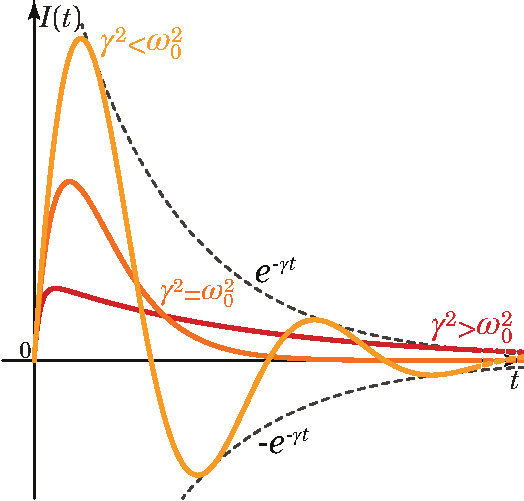
\includegraphics[width=0.7\textwidth]{images/chp11/chp11RLCgraf.pdf}
\end{center}
In tutti i tre i casi il passaggio di corrente è dunque soltanto temporaneo, dato che il \textit{fattore di smorzamento} $e^{-\gamma t}$ è prevalente.

\subsection{Circuiti LC}
\begin{define}[Circuito LC]
	Un \textbf{circuito LC}\index{circuito!LC} è un circuito che presenta solo \textit{induttori} e \textit{condensatori}.
	\begin{center}		
		\begin{tikzpicture}[voltage dir=RP]
			\draw (0,0) to [capacitor, C=$C$, v=$V_C$] (0,2.5)
			-- (2.5,2.5)
			to [inductor, L=$L$, v=$\mathcal{E}_i$] (2.5,0)
			to [switch, label=$t<0$, mirror] (0,0)
			-- (0,0.1);
			\draw (1,0) to[short, *-] (1,0);
		\end{tikzpicture}
		\begin{tikzpicture}[voltage dir=RP]
			\draw (0,0) to [capacitor, C=$C$, v=$V_C$, i=$I$] (0,2.5)
			-- (2.5,2.5)
			to [inductor, L=$L$, v=$\mathcal{E}_i$] (2.5,0)
			-- (0,0)
			-- (0,0.1);
			\draw (1,0) to[short, *-] (1,0);
			\node at (1.25,-0.5) {$t>0$};
			\node at (1.25,-0.6) {$ $};
		\end{tikzpicture}
	\end{center}
\end{define}
Sebbene sia una situazione praticamente soltanto teorica (è sostanzialmente impossibile realizzare un circuito di resistenza $R$ nulla!), anche un circuito $LC$ può funzionare \textit{senza la presenza di un generatore}.
Dalla seconda legge di Kirchhoff avremmo che
\begin{align*}
	V_C+V_L=0\\
	\frac{q}{C}-L\dv{I}{t}=0
\end{align*}
L'equazione differenziale che descrive la corrente è
\begin{equation}
		\tcboxmath[colback=yellowpastellow!30!white,drop fuzzy shadow, nobeforeafter, math upper, tcbox raise base, enhanced]{\dv[2]{I}{t}+\omega_0I=0}
\end{equation}
dove $\omega_0$ è la frequenza caratteristica definita precedentemente. In questo caso particolare ci siamo ricondotti all'equazione di un oscillatore armonico \textit{non} smorzato, la cui soluzione è
\begin{equation}
		\tcboxmath[colback=yellowpastellow!30!white,drop fuzzy shadow, nobeforeafter, math upper, tcbox raise base, enhanced]{I(t)=A\sin(\omega_0 t+\oldphi)}
\end{equation}
La differenza di potenziale ai capi del condensatore è la stessa di quella ai capit della induttanza; si ricava facilmente dalla legge di Kirchhoff che essa è $L$ volte la derivata temporale della corrente:
\begin{equation*}
	V_C(t)=V_L(t)=AL\omega_0\cos(\omega_0 t+\oldphi)
\end{equation*}
Determiniamo le costanti di contesto. Sappiamo che la corrente inizia a scorrere soltanto alla chiusura dell'interruttore al tempo $t=0$, mentre la \ddp ai capi del condensatore denotiamola come $V_0=\frac{q}{C}$. Allora
\begin{align*}
	0=I(0)=A\sin(\omega_0 0+\oldphi)=A\sin(\oldphi)&\implies \oldphi =0\\
	V_0=V_C(0)=AL\omega_0\cos(\omega_0 0+\oldphi)=AL\omega_0\cos(\oldphi)=AL\omega_0&\implies A=\frac{V_0}{L\omega_0}
\end{align*}
Le equazioni diventano dunque
\begin{empheq}[box=\tcmathboxgeneral]{align}
	I(t)&=\frac{V_0}{L\omega_0}\sin(\omega_0 t)\\
	V_C(t)&=V_L(t)=V_0\cos(\omega_0 t)
\end{empheq}
\paragraph{Corrente continua e alternata}
Fino ad ora avevamo incontrato circuiti dotati di generatori che chiamiamo a corrente \textit{continua}: come le batterie o altri di natura elettrochimica, essi producono una corrente potenzialmente variabile nel tempo, ma che non cambia mai direzione nel conduttore.
\begin{define}[Corrente continua]
	La corrente elettrica è detta \textbf{continua}\index{corrente elettrica!continua} (DC) se la sua direzione è costante; la sua intensità può essere anch'essa costante oppure può variare d'intensità nel tempo. 
\end{define}
Con il circuito $LC$ siamo di fronte ad una situazione nuova: la \ddp del circuito e la corrente non solo variano nel tempo, ma hanno un comportamento \textit{sinusoidale}. Chiamiamo tale tipo di corrente \textit{alternata}.\\
In Fisica, parliamo di \textit{grandezze alternate} se sono periodiche e hanno un valor medio nullo in un periodo; nell'uso comune il termine è riservato soltanto alle variazioni sinusoidali.
\begin{define}[Corrente alternata]
	La corrente elettrica è detta \textbf{alternata}\index{corrente elettrica!alternata} (AC) se è una grandezza alternata: il valor medio della corrente è nullo e varia intensità e direzione periodicamente.
\end{define}
\paragraph{L'andamento periodico}
Sia $T$ il periodo dell'oscillazione; cosa succede nel circuito in tale periodo?
\begin{itemize}
	\item La corrente parte nulla, mentre la \ddp ai capi del condensatore è massima
	\begin{align*}
		I(t=0)&=0\\
		V_C(t=0)&=V_0
	\end{align*}
	\item Man mano che il condensatore si \textit{scarica}, la corrente aumenta fino a raggiungere il valore massimo e la \ddp ad annullarsi. Allo stesso tempo la variazione di corrente induce sia l'induttore a produrre una corrente di verso opposto, sia ad immagazzinare energia magnetica. Ad un quarto del periodo il condensatore è scarico, mentre l'induttore è completamente carico.
	\begin{align*}
	 	I\left(t=\dfrac{T}{4}\right)&=I_{max}\\
	 	V_C\left(t=\dfrac{T}{4}\right)&=0
	 \end{align*}
	\item Superato $t=\nicefrac{T}{4}$, il condensatore inizia a ricaricarsi e la \ddp ai capi del condensatore si inverte di segno. Dopo mezzo periodo, il condensatore è tornato carico mentre l'induttore non ha più energia; in particolare, la corrente è di nuovo nulla e la \ddp è massima, ma di segno opposto.
	\begin{align*}
		I\left(t=\dfrac{T}{2}\right)&=0\\
		V_C\left(t=\dfrac{T}{2}\right)&=-V_0
	\end{align*}
	\item Superato $t=\nicefrac{T}{2}$, riparte il processo di scarica del condensatore e di carica dell'induttore; questa volta, la corrente percorre il verso opposto di quello di partenza e incrementa la sua intensità fino a raggiungere il massimo negativo a tre quarti del periodo. La \ddp decresce fino ad annullarsi.
	\begin{align*}
		I\left(t=\dfrac{3}{4}T\right)&=-I_{max}\\
		V_C\left(t=\dfrac{3}{4}T\right)&=0
	\end{align*}
	\item Nell'ultimo quarto di periodo il condensatore si carica, l'induttore si scarica e la situazione torna quella di partenza.
\end{itemize}
Da quanto osservato, possiamo affermare che $I$ e $V_C$ sono in \textbf{quadratura di fase}\index{quadratura di fase}: quando la corrente è massima $V_C$ è nulla e viceversa.
\begin{center}
	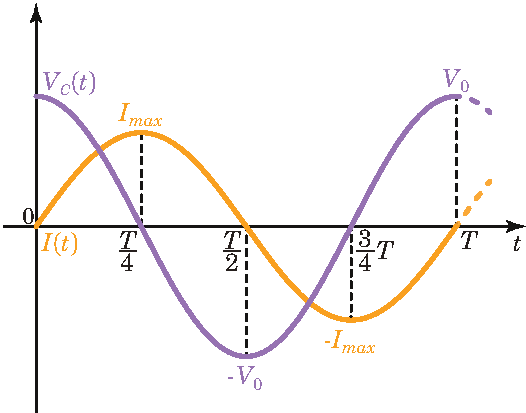
\includegraphics[width=0.7\textwidth]{images/chp11/chp11LCgraf.pdf}
\end{center}
\paragraph{Energia del circuito RLC}
Si può notare che l'andamento della corrente e della differenza di potenziale comporta un'oscillazione tra l'\textit{energia} del \textit{campo elettrico}, immagazzinata nel \textit{condensatore}...
\begin{equation*}
	U_C(t)=\frac{CV^2_C(t)}{2}
\end{equation*}
... e l'\textit{energia} del \textit{campo magnetico}, immagazzinata nell'\textit{induttore}.
\begin{equation*}
	U_L(t)=\frac{LI^2(t)}{2}
\end{equation*}
Sono anch'esse in \textit{quadratura di fase}! Quando la corrente è massima (e la \ddp nulla) l'energia del circuito è soltanto magnetica (perché quella elettrica è zero) e viceversa. In ogni caso, per \textit{conservazione dell'energia}, l'energia totale è quella del condensatore alla chiusura dell'interrutore a $t=0$ o a quella dell'induttore a metà periodo:
\begin{equation}
	\tcboxmath[colback=yellowpastellow!30!white,drop fuzzy shadow, nobeforeafter, math upper, tcbox raise base, enhanced]{E_{tot}=\frac{CV^2_C(t)}{2}+\frac{LI(t)^2}{2}=\frac{1}{2}CV_0^2=\frac{1}{2}LI_0^2}
\end{equation}
\section{Elettrogeneratori}
\begin{define}[Elettrogeneratore]
	Un \textbf{elettrogeneratore}\index{elettrogeneratore} è un dispositivo elettrotecnico che converte \textit{energia meccanica} in \textit{energia elettrica}.
\end{define}
\subsection{Spira mobile}\label{spiramobilegeneratori}
Un esempio facile - ma di scarsa rilevanza pratica - di \textit{elettrogeneratore} è quello di una \textbf{spira mobile}\index{spira!mobile}. Consideriamo un circuito a forma di U \textit{aperto} e di altezza $h$, come in figura.
\begin{center}
	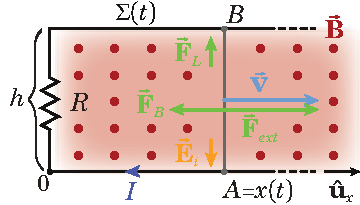
\includegraphics[width=0.4\textwidth]{images/chp11/chp11generatorespira.pdf}
\end{center}
Esso è fisso e immerso in un campo magnetico $\vba{B}$ uniforme e perpendicolare ad esso. Sui rami laterali, nel punto $x$ è posto una \textit{sbarra conduttrice rigida} di lunghezza $h$; essa è libera di muoversi lungo i rami - la posizione è $x=x(t)$. Il circuito assieme alla sbarra formano una spira chiusa $\Sigma$.\\
Inizialmente nel circuito non è presente una corrente, ma appena muoviamo la sbarra con velocità $\vba{v}$, dovuta ad un'azione esterna, l'area $\Sigma$ della spira \textit{cambia} e di conseguenza cambia il flusso del campo magnetico attraverso di essa. Dalla legge di Faraday-Neumann-Lenz la \fem indotta è
\begin{equation*}
	\mathcal{E}_i=-\dv{\Phi_{\Sigma}(\vba{B})}{t}
\end{equation*}
Poiché l'area della spira è
\begin{equation*}
	\Sigma(t)=hx(t)
\end{equation*}
il flusso è, data la perpendicolarità del campo magnetico alla spira, pari a
\begin{equation*}
	\Phi_{\Sigma}(\vba{B})=B\Sigma(t)=Bhx(t)
\end{equation*}
La variazione della posizione $x(t)$ nel tempo è la velocità $\vba{v}$ con cui viene sposta la spira, pertanto
\begin{equation*}
	\mathcal{E}_i=-\dv{\Phi_{\Sigma}(\vba{B})}{t}=-B\dv{\Sigma(t)}{t}=-Bh\dv{x(t)}{t}=-Bhv
\end{equation*}
\begin{equation}
	\tcboxmath[colback=yellowpastellow!30!white,drop fuzzy shadow, nobeforeafter, math upper, tcbox raise base, enhanced]{\mathcal{E}_i=-Bhv}
\end{equation}
\begin{observe}
	Come abbiamo affermato nel \autoref{chap:elettromagnetismoTempo}, sezione \ref{faradayavevaascopertoiltempo}, pag. \pageref{faradayavevaascopertoiltempo}, la creazione di una \fem indotta in questo caso (deformazione di una spira) si poteva anche ricavare nota la \textit{sola} forza di Lorentz.\\
	Muovendo la filo, le cariche libere in esso si muovono solidali alla sbarra e quindi subiscono una forza di Lorentz
	\begin{equation*}
		\vba{F}_L=e\vba{v}\cross\vba{B}
	\end{equation*}
	e di conseguenza generano un campo elettrico indotto
	\begin{equation*}
		\vba{E}_i=\frac{\vba{F}_L}{e}=\vba{v}\cross\vba{B}
	\end{equation*}
	La \fem indotta si ricava dalla definizione di forza elettromotrice come circuitazione:
	\begin{equation*}
		\mathcal{E}_i=\oint \vba{E}_i\vdot d\vba{s}=\int_{B}^{A}\vba{E}_i\vdot d\vba{s}=-Bv\int_{A}^{B}ds=-Bhv
	\end{equation*}
\end{observe}
Supponendo che la parte fissa abbia una resistenza $R$, dalla \textit{legge di Ohm} la corrente che circola nel circuito è
\begin{equation}
	\tcboxmath[colback=yellowpastellow!30!white,drop fuzzy shadow, nobeforeafter, math upper, tcbox raise base, enhanced]{I=\frac{\abs{\mathcal{E}_i}}{R}=\frac{Bhv}{R}}
\end{equation}
\begin{observe}
	La corrente indotta, per la legge di Lenz, deve opporsi al cambio di flusso. Per determinare il verso, possiamo operare diversi metodi, tra cui:
	\begin{itemize}
		\item Dato che la corrente indotta percorrendo la sbarra genera una forza di Laplace $\vba{F}_B$, il verso della corrente deve essere tale che $\vba{F}_B$ si oppone al moto.
		\item Dato che la corrente indotta percorrendo la spira chiusa genera un campo magnetico $\vba{B}_i$, il verso della corrente deve essere tale che $\vba{B}_i$ si oppone a $\vba{B}$.
	\end{itemize}
	Applicandoli entrambi al caso in questione, la corrente dovrà percorrere la spira in \textit{senso orario}.
\end{observe}
\paragraph{Attrito elettromagnetico}
Purtroppo, il moto della spira mobile \textit{non} è privo di attriti. Infatti, il filo percorso dalla corrente autoindotta è soggetto, per la \textit{seconda legge di Laplace}, ad una \textbf{forza di attrito elettromagnetico}\index{forza!di attrito elettromagnetico}
\begin{equation*}
	\vba{F}_B=I\int_{B}^{A}d\vba{s}\cross\vba{B}=-IBh\vbh{u}_x=-\frac{h^2B^2}{R}\vba{v}
\end{equation*}
\begin{equation}
	\tcboxmath[colback=yellowpastellow!30!white,drop fuzzy shadow, nobeforeafter, math upper, tcbox raise base, enhanced]{\vba{F}_B=-\frac{h^2B^2}{R}\vba{v}}
\end{equation}
che, naturalmente, si oppone al moto.
\begin{observe}
	La forza di attrito assume la forma di un \textit{attrito viscoso}, in quanto è proporzionale alla velocità.
\end{observe}
Per mantenere una velocità costante $\vba{v}$ dobbiamo applicare alla sbarra una \textit{forza esterna} uguale e contraria a quella dell'\textit{attrito elettromagnetico}.
\begin{equation*}
	\vba{F}_{ext}=-\vba{F}_B
\end{equation*}
È necessario compiere un \textit{lavoro} per mantenere tale equilibrio o, in altri termini, devo produrre un'opportuna \textit{potenza meccanica} da sopperire alla \textit{potenza elettrica} dissipata dalla resistenza per avere la corrente elettrica nel circuito.
Nel caso della spira mobile, essa è
\begin{equation}
	\tcboxmath[colback=yellowpastellow!30!white,drop fuzzy shadow, nobeforeafter, math upper, tcbox raise base, enhanced]{P=\vba{F}_{ext}\vdot \vba{v}=\frac{h^2B^2v}{R}=I^2R}
\end{equation}
\subsection{Disco di Barlow}
Come generatore, la spira mobile non è particolarmente funzionale: per continuare a produrre corrente dovrei avere delle \textit{rotaie infinite} su cui far scorrere la sbarra. Per produrre una corrente è nettamente più efficace ricorrere a sistemi che utilizzano energia meccanica di natura \textit{rotazionale}; la \textbf{ruota di Barlow}\index{ruota di Barlow} o \textbf{disco di Barlow}\index{disco di Barlow} è uno dei primi. Esso consiste in un disco di materiale conduttore che ruota attorno al suo asse con velocità angolare costante $\omega$, dovuta ad un'azione esterna.
\begin{center}
	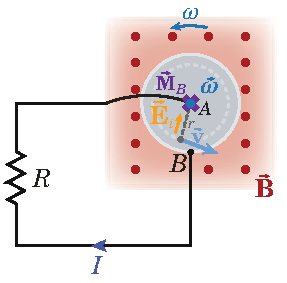
\includegraphics[width=0.4\textwidth]{images/chp11/chp11generatorediscodibarlow.pdf}
\end{center}
\begin{observe}
	Il vettore velocità angolare $\vba{\omega}$ è perpendicolare al disco e il verso è dato da una \textit{variante} della \textit{regola della mano destra}: curvando le dita della mano in modo che le dita della mano seguano la direzione di rotazione - oraria o antioraria - il pollice retto punta nel verso di $\vba{\omega}$.
\end{observe}
Il disco è perpendicolare ad un campo magnetico $\vba{B}$ uniforme uscente dal piano a cui appartiene. Sia l'asse (punto $A$), sia la superficie del disco (punto $B$) sono a contatto di due elementi striscianti collegati ad un elemento di resistenza $R$ - di fatto rendendo il sistema complessivo funzionalmente una spira.
La variazione della velocità del disco va a creare una variazione del flusso del campo magnetico e dunque una \ddp indotta ai capi $A$ e $B$ del circuito.
Ricordiamo che possiamo descrivere la posizione di un punto sul disco in coordinate polari\label{femdiscobarlow}
\begin{equation*}
	\vba{r}=(r\cos\phi,r\sin\phi)
\end{equation*}
dove $r$ è la distanza dall'asse e $\phi$ l'angolo di rotazione rispetto all'asse $x$ di un sistema di riferimento cartesiano opportunamente scelto. La velocità di tale punto è data da
\begin{align*}
	\vba{v}&=\dv{r}{t}=\\
	&=\left(\dot{r}\cos\phi-\dot{\phi}r\sin\phi,\dot{r}\sin\phi+\dot{\phi}r\cos\phi\right)=\\
	&=\dot{r}\left(\cos\phi,\sin\phi\right)+\dot{\phi}r\left(-\sin\phi,\cos\phi\right)=\\
	&=\dot{r}\vbh{u}_r+\dot{\phi}r\vbh{u}_{\phi}
\end{align*}
Se consideriamo una carica libera nel disco a distanza $r$ dall'asse, essa ruota solidale con il disco alla stessa velocità angolare $\vba{\omega}$ e si muove dunque su traiettorie circolari; poiché non varia il raggio $r$, si ha $\dot{r}=0$ e la velocità subita è soltanto una tangenziale e non radiale.
\begin{equation*}
	\vba{v}=\dot{\phi}r\vbh{u}_{\phi}=\dv{\phi}{t}r\vbh{u}_{\phi}=\omega r\vbh{u}_{\phi}
\end{equation*}
Il campo elettrico indotto a distanza $r$ dall'asse è quindi
\begin{equation*}
	\vba{E}_i=\vba{v}\cross\vba{B}=\dv{\phi}{t}r\vbh{u}_{\phi}\cross\vba{B}=\omega r\vbh{u}_{\phi}\cross\vba{B}=-\omega r B\vbh{u}_r
\end{equation*}
Allora la forza elettromotrice è, dalla definizione come circuitazione, 
\begin{equation*}
	\mathcal{E}_i=\int_{A}^{B}\vba{E}_i\vdot d\vba{s}=\int_{B}^{A}\omega r' B\vbh{u}_r\vdot d\vba{s}=\omega B\int_0^a r'dr'=\frac{1}{2}\omega Ba^2
\end{equation*}
\begin{equation}
	\tcboxmath[colback=yellowpastellow!30!white,drop fuzzy shadow, nobeforeafter, math upper, tcbox raise base, enhanced]{\mathcal{E}_i=\frac{1}{2}\omega Ba^2}
\end{equation}
dove $a$ è il raggio del disco; la corrente è
\begin{equation}
	\tcboxmath[colback=yellowpastellow!30!white,drop fuzzy shadow, nobeforeafter, math upper, tcbox raise base, enhanced]{I=\frac{\mathcal{E}_i}{R}=\frac{\omega B a^2}{2R}}
\end{equation}
\paragraph{Attrito elettromagnetico torcente}
Sull'elemento radiale infinitesimo\footnote{Il segno è scelto positivo in quanto l'orientazione di $d\vba{s}$ segue quello della corrente $I$, ossia concorde al versore radiale dal centro del disco.} $d\vba{s}=-ds\vbh{u}_r$ a distanza $\vba{r}=s\vbh{u}_r$ dal centro, percorso da corrente $I$, agisce una forza (infinitesima) di Laplace
\begin{equation*}
	d\vba{F}_B=I d\vba{s}\cross \vba{B}=\frac{\omega B a^2}{2R}d\vba{s}\cross \vba{B}=\frac{\omega B^2 a^2}{2R}ds\vbh{u}_r\cross \vbh{u}_z=-\frac{\omega B^2 a^2}{2R} ds\vbh{u}_{\phi}
\end{equation*}
che, rispetto all'asse, ha momento (infinitesimo)
\begin{equation*}
	d\vba{M}_B=\vba{r}\cross d\vba{F}_B=-\frac{\omega B^2 a^2}{2R}ds\vba{r}\cross\vbh{u}_{\phi}=-\frac{\omega B^2 a^2}{2R}sds\vbh{u}_r\cross\vbh{u}_{\phi}=-\frac{\omega B^2 a^2}{2R}s\ ds\vbh{u}_{z}=-\frac{B^2a^2}{2R}sds\vba{\omega}
\end{equation*}
Il disco è soggetto dunque ad un \textit{momento magnetico} ortogonale e opposto a $\vba{\omega}$:
\begin{equation*}
	\vba{M}_B=\int_{B}^{A}d\vba{M}_B=I\int_{B}^{A}\vba{r}\cross(d\vba{s}\cross\vba{B})=-\frac{B^2a^2}{2R}\int_{0}^{a}sds\vba{\omega}=-\frac{B^2a^4}{4R}\vba{\omega}
\end{equation*}
\begin{equation}
	\tcboxmath[colback=yellowpastellow!30!white,drop fuzzy shadow, nobeforeafter, math upper, tcbox raise base, enhanced]{\vba{M}_B=-\frac{IBa^2}{2}\vbh{u}_z=-\frac{B^2a^4}{4R}\vba{\omega}}
\end{equation}
Questo momento risulta essere un \textit{attrito torcente} che si oppone alla velocità angolare. Per mantenere $\omega$ costante bisogna applicare al disco un \textit{momento esterno} uguale e contrario a questo \textbf{attrito elettromagnetico torcente}.
\begin{equation*}
	\tcboxmath[colback=yellowpastellow!30!white,drop fuzzy shadow, nobeforeafter, math upper, tcbox raise base, enhanced]{\vba{M}_{ext}=-\vba{M}_B}
\end{equation*}
La \textit{potenza meccanica} per mantenere l'equilibrio e sopperire alla \textit{potenza elettrica} dissipata dalla resistenza è
\begin{equation}
	\tcboxmath[colback=yellowpastellow!30!white,drop fuzzy shadow, nobeforeafter, math upper, tcbox raise base, enhanced]{P=\vba{M}_{ext}\vdot\vba{\omega}=\frac{B^2a^4\omega^2}{4R}=I^2R}
\end{equation}
\subsection{Generatori di corrente alternata}
Consideriamo una \textit{spira} piana immersa in un campo magnetico $\vba{B}$ uniforme. La spira ruota con velocità angolare $\omega$ uniforme attorno al suo asse verticale in senso orario; pertanto, il flusso del campo magnetico tramite essa varia e, per la legge di Faraday-Neumann-Lenz, varia anche la \fem indotta:
\begin{equation*}
	\mathcal{E}_i=-\dv{\Phi_{\Sigma}(\vba{B})}{t}
\end{equation*}
La variazione di flusso dipende dall'angolo $\alpha$ tra $\vba{B}$ e la normale alla spira:
\begin{equation*}
	\cos\alpha=\vba{B}\vdot\vbh{u}_n
\end{equation*}
Poiché la spira ruota con velocità angolare uniforme, significa che
\begin{equation*}
	\alpha(t)=\omega t+\oldphi
\end{equation*}
dove $\oldphi$ dipende dalle condizioni iniziali. Si ha
\begin{equation*}
	\Phi_{\Sigma}(\vba{B})=\vba{B}\vdot\vbh{u}_n\Sigma=\Sigma B\cos(\omega t+\oldphi)
\end{equation*}
da cui segue
\begin{equation}
	\tcboxmath[colback=yellowpastellow!30!white,drop fuzzy shadow, nobeforeafter, math upper, tcbox raise base, enhanced]{\mathcal{E}_i(t)=-\dv{\Phi_{\Sigma}(\vba{B})}{t}=\Sigma B\omega\sin(\omega t+\oldphi)}
\end{equation}
Notiamo che la \fem varia \textit{sinusoidalmente nel tempo}, con valore massimo assunto 
\begin{equation}
	\tcboxmath[colback=yellowpastellow!30!white,drop fuzzy shadow, nobeforeafter, math upper, tcbox raise base, enhanced]{\mathcal{E}_{max}=\Sigma B\omega}
\end{equation}
\begin{center}
	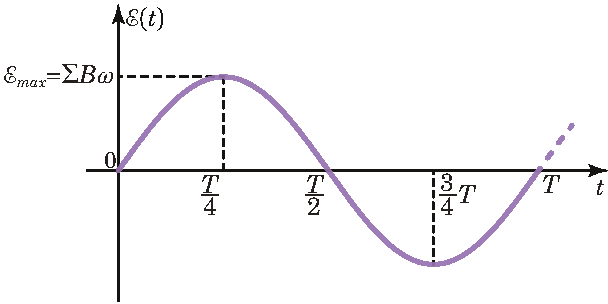
\includegraphics[width=0.7\textwidth]{images/chp11/chp11ddpgeneratoriACgraf.pdf}
\end{center}
La corrente elettrica che scorre nel circuito è
\begin{equation}
	\tcboxmath[colback=yellowpastellow!30!white,drop fuzzy shadow, nobeforeafter, math upper, tcbox raise base, enhanced]{I(t)=\frac{\Sigma B\omega}{R}\sin(\omega t+\oldphi)}
\end{equation}
e, come la \fem che la genera, varia \textit{sinusoidalmente nel tempo}, con valore massimo 
\begin{equation}
	\tcboxmath[colback=yellowpastellow!30!white,drop fuzzy shadow, nobeforeafter, math upper, tcbox raise base, enhanced]{I_{max}=\frac{\Sigma B\omega}{R}}
\end{equation}
\begin{center}
	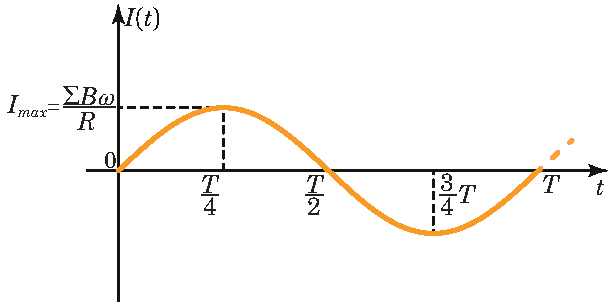
\includegraphics[width=0.7\textwidth]{images/chp11/chp11corgeneratoriACgraf.pdf}
\end{center}
La corrente elettrica risulta cambiare verso periodicamente ed è quindi una \textit{corrente alternata}.\\ 
Anche la \textit{potenza elettrica} varia periodicamente nel tempo, rimanendo però per ovvi motivi sempre una quantità positiva:
\begin{equation}
	\tcboxmath[colback=yellowpastellow!30!white,drop fuzzy shadow, nobeforeafter, math upper, tcbox raise base, enhanced]{P(t)=\mathcal{E}_i I=\frac{\mathcal{E}_i^2}{R}=\frac{B^2\Sigma^2\omega^2}{R}\sin^2(\omega t)=\vba{M}\cdot \vba{\omega}=M\omega}
\end{equation}
dove $M(t)$ è il momento magnetico della spira. Il valore massimo è
\begin{equation}
	\tcboxmath[colback=yellowpastellow!30!white,drop fuzzy shadow, nobeforeafter, math upper, tcbox raise base, enhanced]{P_{max}=\mathcal{E}_{max}I_{max}=\frac{\mathcal{E}_{max}^2}{R}=\frac{B^2\Sigma^2\omega^2}{R}}
\end{equation}
\begin{center}
	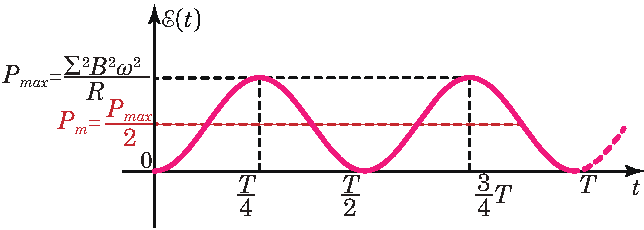
\includegraphics[width=0.7\textwidth]{images/chp11/chp11potgeneratoriACgraf.pdf}
\end{center}
\paragraph{Potenza e f.e.m. efficace}
Nella pratica, tuttavia, il periodo dell'elettrogeneratore è \textit{talmente breve} che i valori della potenza e della \fem oscillano così furiosamente da rendere impraticabile uno studio dei loro valori al variare del tempo. Ci interessa quindi approssimare un generatore AC ad uno a corrente continua sostanzialmente equivalente. Dato che lo scopo principale dei generatori è quello di convertire un energia meccanica in energia elettrica, possiamo cercare un elettrogeneratore DC che produca una potenza uguale a quella che, \textit{mediamente}, il generatore AC produce. Tale potenza elettrica deve valere
\begin{equation}
	\tcboxmath[colback=yellowpastellow!30!white,drop fuzzy shadow, nobeforeafter, math upper, tcbox raise base, enhanced]{P_m=\frac{1}{T}\int_0^{t}P(t)dt=\frac{B^2\Sigma^2\omega^2}{R}\int_0^{t}\sin^2\omega tdt=\frac{B^2\Sigma^2\omega^2}{2R}=\frac{P_{max}}{2}=\frac{\mathcal{E}_{max}^2}{2R}}
\end{equation}
Il generatore DC sostitutivo deve quindi produrre una \fem $\mathcal{E}_{eff}$, detta \textbf{forza elettromotrice efficace}\index{forza elettromotrice!effficace}, tale per cui
\begin{equation}
	\tcboxmath[colback=yellowpastellow!30!white,drop fuzzy shadow, nobeforeafter, math upper, tcbox raise base, enhanced]{P_m=\frac{\mathcal{E}^2_{eff}}{R}}
\end{equation}
ossia
\begin{equation*}
	\frac{\mathcal{E}_{max}^2}{2R}=\frac{\mathcal{E}^2_{eff}}{R}
\end{equation*}
\begin{equation}
	\tcboxmath[colback=yellowpastellow!30!white,drop fuzzy shadow, nobeforeafter, math upper, tcbox raise base, enhanced]{\mathcal{E}_{eff}=\frac{\mathcal{E}_{max}}{\sqrt{2}}}
\end{equation}
\pagebreak
\section{Motori}
\begin{define}[Motore]
	Un \textbf{motore}\index{motore} è un dispositivo elettrotecnico che converte \textit{energia elettrica} in \textit{energia meccanica}.
\end{define}
\subsection{Spira mobile}
Consideriamo una spira simile a quella di pag. \pageref{spiramobilegeneratori}, ma invece di immergerla in un campo magnetico supponiamo di porre nel circuito un generatore di \fem $\mathcal{E}_0$ dotato di una resistenza non trascurabile $R$: esso genera una corrente che circola nella spira e, in particolare, sulla sbarra scorrevole.
\begin{center}
	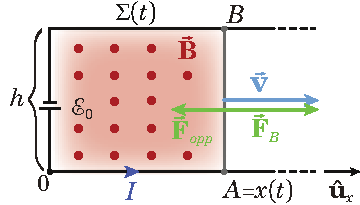
\includegraphics[width=0.4\textwidth]{images/chp11/chp11motorespira.pdf}
\end{center}
Per la \textit{seconda legge di Laplace}, su di essa agisce una forza
\begin{equation*}
	\vba{F}_B=I\left(\int_{A}^{B}d\vba{s}\right)\cross\vba{B}=IBh\vbh{u}_x
\end{equation*}
che fa spostare la barra con una velocità $\vba{v}(t)$. Poiché essa si muove, il flusso del campo magnetico tramite la superficie varia e produce per la legge di Faraday-Neumann-Lenz una \fem indotta nella spira che, come già visto, è pari a
\begin{equation*}
	\mathcal{E}_{i}=-vhB
\end{equation*}
e si contrappone a $\mathcal{E}_0$. Siamo dunque in presenza di un fenomeno di \textit{autoinduzione}: nella spira circola complessivamente una corrente
\begin{equation}
	\tcboxmath[colback=yellowpastellow!30!white,drop fuzzy shadow, nobeforeafter, math upper, tcbox raise base, enhanced]{I=\frac{\mathcal{E}_0-\mathcal{E}_i}{R}=\frac{\mathcal{E}_0-vhB}{R}}
\end{equation}
Supponiamo inoltre che sia presente una \textit{forza} $\vba{F}_{opp}$ opposta al moto $\vba{v}$, rappresentante ad esempio un corpo da trainare attaccato all'asta. La forza complessiva sulla sbarra è
\begin{equation*}
	\vba{F}=\vba{F}_B-\vba{F}_{opp}=\left(IhB-F_{opp}\right)\vbh{u}_x=\left(\frac{\mathcal{E}_0-vhB}{R}hB-F_{opp}\right)\vbh{u}_x
\end{equation*}
\begin{observe}
	Nella forza indotta $\vba{F}_i$ è presente una componente resistiva simile all'\textit{attrito elettrostatico}:
	\begin{equation*}
		\vba{F}_A=-\frac{h^2B^2}{R}\vba{v}
	\end{equation*}
\end{observe}
Dalla legge di Newton abbiamo che
\begin{align*}
	&\vba{F}=m\vba{a}=m\dv{\vba{v}}{t}\\
	&\left(\frac{\mathcal{E}_0-vhB}{R}hB-F_{opp}\right)\vbh{u}_x=m\dv{v}{t}\vbh{u}_x
\end{align*}
Da cui, riordinando i termini, otteniamo un'equazione differenziale ordinaria
\begin{equation*}
	\dv{v}{t}+\frac{h^2B^2}{mR}v+\left(\frac{F_{opp}}{m}-\frac{\mathcal{E}_0}{mR}\right)=0
\end{equation*}
la cui soluzione è
\begin{equation}
	\tcboxmath[colback=yellowpastellow!30!white,drop fuzzy shadow, nobeforeafter, math upper, tcbox raise base, enhanced]{v(t)=\left(\frac{\mathcal{E}_0}{hB}-\frac{R F_{opp}}{h^2B^2}\right)\left(1-e^{-\frac{h^2B^2}{mR}t}\right)}
\end{equation}
\begin{center}
	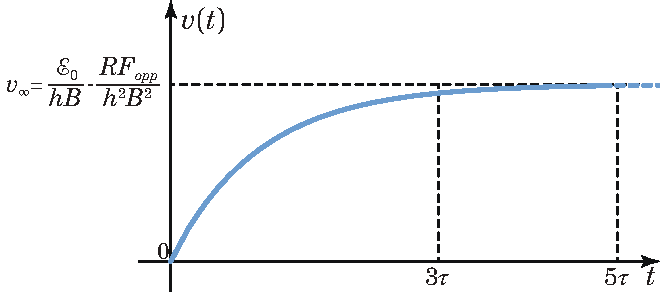
\includegraphics[width=0.7\textwidth]{images/chp11/chp11velmotoreACgraf.pdf}
\end{center}
L'andamento temporale della velocità è dettato dal \textit{tempo caratteristico}:
\begin{equation}
	\tcboxmath[colback=yellowpastellow!30!white,drop fuzzy shadow, nobeforeafter, math upper, tcbox raise base, enhanced]{\tau=\frac{mR}{B^2h^2}}
\end{equation}
Essa è una costante dimensionalmente pari ad una quantità temporale e quindi nel SI si misura in secondi:
\begin{equation*}
	\left[\tau\right]=\frac{\left[m\right]\left[R\right]}{\left[B\right]^2\left[h\right]^2}=\mathsf{M}\cdot\mathsf{M}\mathsf{L}^2\mathsf{T}^{-3} \mathsf{I}^{-2}\cdot \mathsf{M}^{-2} \mathsf{I}^{2} \mathsf{T}^4\cdot\mathsf{L}^{-2}  =\mathsf{T}
\end{equation*}
La velocità della sbarra dopo un tempo \textit{infinito} (ossia a \textit{regime}) è costante e la forza applicata è nulla in quanto $F_B=F_{opp}$; tale velocità è pari a
\begin{equation}
	\tcboxmath[colback=yellowpastellow!30!white,drop fuzzy shadow, nobeforeafter, math upper, tcbox raise base, enhanced]{v_{\infty}=\frac{\mathcal{E}_0}{hB}-\frac{R F_{opp}}{h^2B^2}}
\end{equation}
da cui segue che la \fem, la corrente e la potenza di regime sono
\begin{empheq}[box=\tcmathboxgeneral]{align}
	\mathcal{E}_i&=-\mathcal{E}_0+\frac{R F_{opp}}{hB}\\
	I_{\infty}&=\frac{F_{opp}}{hB}\\
	P_{\infty}&=RI_{\infty}^2+F_{opp}v_{\infty}
\end{empheq}
Il primo termine della potenza di regime è la potenza dissipata dalla resistenza, mentre il secondo è la potenza meccanica necessaria a vincere la forza resistente $\vba{F}_{opp}$.
\subsection{⋆ Disco di Barlow}
In modo analogo a quanto visto con la spira mobile, consideriamo un disco di Barlow di raggio $r$ in cui al posto del resistore è posto un generatore di \fem $\mathcal{E}_0$ che deve vincere un momento meccanico esterno $\vba{M}_{opp}$, che può rappresentare ad esempio una fune che sostiene una massa.
\begin{center}
	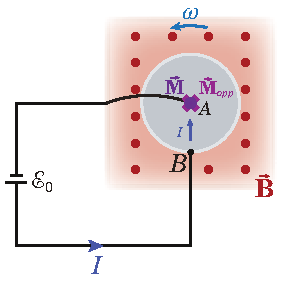
\includegraphics[width=0.4\textwidth]{images/chp11/chp11motorediscodibarlow.pdf}
\end{center}
Sull'elemento radiale infinitesimo\footnote{Il segno è scelto negativo in quanto l'orientazione di $d\vba{s}$ segue quello della corrente $I$, ossia concor al versore radiale dal centro del disco.} $d\vba{s}=-ds\vbh{u}_r$ a distanza $\vba{r}=s\vbh{u}_r$ dal centro, percorso da corrente $I$, agisce una forza (infinitesima) di Laplace
\begin{equation*}
	d\vba{F}_B=I d\vba{s}\cross \vba{B}=-IBds\vbh{u}_r\cross \vbh{u}_z=IBds\vbh{u}_{\phi}
\end{equation*}
che, rispetto all'asse, ha momento (infinitesimo)
\begin{equation*}
	d\vba{M}_B=\vba{r}\cross d\vba{F}_B=I\vba{r}\cross\left(d\vba{s}\cross \vba{B}\right)=IBds\vba{r}\cross\vbh{u}_{\phi}=IBsds\vbh{u}_r\cross\vbh{u}_{\phi}=IBsds\vbh{u}_{z}
\end{equation*}
Il disco è soggetto dunque ad un \textit{momento magnetico} ortogonale
\begin{equation*}
	\vba{M}_B=\int_{B}^{A}d\vba{M}_B=I\int_{B}^{A}\vba{r}\cross(d\vba{s}\cross\vba{B})=IB\int_{0}^{a}sds\vbh{u}_{z}=\frac{IBa^2}{2}\vbh{u}_{z}
\end{equation*}
\begin{equation}
	\tcboxmath[colback=yellowpastellow!30!white,drop fuzzy shadow, nobeforeafter, math upper, tcbox raise base, enhanced]{\vba{M}_B=\frac{IBa^2}{2}\vbh{u}_{z}}
\end{equation}
che fa ruotare il disco con velocità angolare (vettoriale) $\vba{\omega}$ parallela e concorde a $\vba{M}_B$. Si può mostrare in modo assolutamente analogo a quanto fatto a  pag. \pageref{femdiscobarlow} che tale rotazione, per la \textit{legge di Faraday-Neumann-Lenz} produce una \fem indotta
\begin{equation*}
	\tcboxmath[colback=yellowpastellow!30!white,drop fuzzy shadow, nobeforeafter, math upper, tcbox raise base, enhanced]{\mathcal{E}_i=\frac{1}{2}\omega Ba^2}
\end{equation*}
tale per cui nel sistema circola una corrente complessiva
\begin{equation*}
	I=\frac{\mathcal{E}_0-\mathcal{E}_i}{R}=\frac{\mathcal{E}_0-\frac{1}{2}\omega Ba^2}{R}
\end{equation*}
Dal \textit{teorema del momento angolare} otteniamo l'equazione differenziale ordinaria che descrive il moto:
\begin{equation*}
	\mathbf{I}\dv{\omega}{t}=M_B-M_{opp}\frac{IBr^2}{2}-M_{opp}
\end{equation*}
con $\mathbf{I}$ il momento di inerzia del disco rispetto all'asse di rotazione.\\
L'andamento temporale della velocità è dettato dal \textit{tempo caratteristico}:
\begin{equation}
	\tcboxmath[colback=yellowpastellow!30!white,drop fuzzy shadow, nobeforeafter, math upper, tcbox raise base, enhanced]{\tau=\frac{4\mathbf{I}R}{B^2}}
\end{equation}
che, come tutti i tempi caratteristici visti finora, si vede essere dimensionalmente (poco) sorprendentemente pari ad una quantità temporale - quindi nel SI si misura in secondi.\\
La velocità angolare della sbarra dopo un tempo \textit{infinito} (ossia a \textit{regime}) è costante e il momento complessivo è nullo in quanto $M_B=M_{opp}$; essa è pari a
\begin{equation}
	\tcboxmath[colback=yellowpastellow!30!white,drop fuzzy shadow, nobeforeafter, math upper, tcbox raise base, enhanced]{\omega_{\infty}=\frac{2}{Br^2}\left(\mathcal{E}_0-\frac{2RM_{opp}}{Br^2}\right)}
\end{equation}
da cui segue che la \fem, la corrente e la potenza di regime sono
\begin{empheq}[box=\tcmathboxgeneral]{align}
	\mathcal{E}_i&=-\mathcal{E}_0+\frac{2R M_{opp}}{Ba^2}\\
	I_{\infty}&=\frac{2M_{opp}}{Ba^2}\\
	P_{\infty}&=RI_{\infty}^2+M_{opp}\omega_{\infty}
\end{empheq}
\section{Il metodo simbolico}
Finché ci limitiamo a \textit{circuiti semplici}, costituiti solo da un generatore AC e un componente elettrico, determinare tutte le grandezze in gioco non è particolarmente difficile. Tuttavia, in presenza di \textit{molte componenti} risulta particolarmente complicato - dato che stiamo operando con grandezze sinusoidali!\\
In aiuto ci viene il \textbf{metodo simbolico}\index{metodo simbolico}, un approccio di analisi dei circuiti che consente di risolvere le reti in corrente alternata sinusoidale in modo formalmente analogo alle reti in corrente continua grazie ai \textit{fasori}\footnote{Nelle ``Note aggiuntive'', a pag. \pageref{fasori}, è possibile trovare maggiori dettagli e risultati sui fasori.}. L'idea di fondo è di associare all'intensità di corrente
\begin{equation}
	I(t)=I_0\cos(\omega t+\oldphi_I)
\end{equation}
un'\textbf{intensità di corrente complessa}\index{intensità di corrente complessa}, ossia il fasore
\begin{equation}
	\tcboxmath[colback=yellowpastellow!30!white,drop fuzzy shadow, nobeforeafter, math upper, tcbox raise base, enhanced]{\hat{I}(t)=I_0\cos(\omega t+\oldphi_I)+iI_0\sin(\omega t+\oldphi_I)=I_0e^{i(\omega t+\oldphi_I)}=I_0e^{i\omega t}e^{i\oldphi_I}}
\end{equation}
in modo che la parte reale della corrente complessa sia la corrente vera e propria
\begin{equation}
	\tcboxmath[colback=yellowpastellow!30!white,drop fuzzy shadow, nobeforeafter, math upper, tcbox raise base, enhanced]{\Re{\hat{I}(t)}=I(t)}
\end{equation}
In modo analogo, alla differenza di potenziale ai capi di una componente elettrica (resistore, induttore, condensatore)
\begin{equation}
	V(t)=V_0\cos(\omega t+\oldphi_V)
\end{equation}
si può definire il fasore associato
\begin{equation}
	\tcboxmath[colback=yellowpastellow!30!white,drop fuzzy shadow, nobeforeafter, math upper, tcbox raise base, enhanced]{\hat{V}(t)=V_0\cos(\omega t+\oldphi_V)+iV_0\sin(\omega t+\oldphi_V)=V_0e^{i(\omega t+\oldphi_V)}=I_0e^{i\omega t}e^{i\oldphi_V}}
\end{equation}
\paragraph{Impedenza  e ammettenza}
Il rapporto tra due fasori qui definiti è una quantità complessa (ma \textit{non} un fasore!) detta \textbf{impedenza elettrica}.
\begin{define}[Impedenza e ammettenza]
	L'\textbf{impedenza elettrica}\index{impedenza!elettrica} è una quantità complessa indipendente dal tempo che rappresenta un ostacolo al passaggio della corrente alternata in un circuito, causando una differenza di potenziale al passaggio di corrente. Essa combina assieme gli effetti di eventuali \textit{resistori}, \textit{induttori} e \textit{condensatori}. La legge che lega l'intensità di corrente e la \ddp è la \textbf{legge di Ohm generalizzata}:
	\begin{equation}
		\tcboxmath[colback=yellowpastellow!30!white,colframe=ceruleancrayola!85!black,drop fuzzy shadow, nobeforeafter, math upper, tcbox raise base, enhanced]{\hat{V}(t)=Z\hat{I}(t)}
	\end{equation}
	Un'espressione dell'impedenza è quindi
	\begin{equation}
		\tcboxmath[colback=yellowpastellow!30!white,colframe=ceruleancrayola!85!black,drop fuzzy shadow, nobeforeafter, math upper, tcbox raise base, enhanced]{Z=\frac{V_0}{I_0}e^{i(\oldphi_V-\oldphi_I)}=\frac{V_0}{I_0}e^{i\theta}}
	\end{equation}
	Il reciproco dell'impedenza è detta \textbf{ammettenza elettrica}\index{ammetenza elettrica}.
	\begin{equation}
		\tcboxmath[colback=yellowpastellow!30!white,colframe=ceruleancrayola!85!black,drop fuzzy shadow, nobeforeafter, math upper, tcbox raise base, enhanced]{
		\mathcal{A}=\frac{1}{Z}}
	\end{equation}
\end{define}
\begin{attention}
	Alcuni testi ambiguamente usano il termine ``\textit{impedenza}'' per indicare il valore reale dato dal \textit{modulo} dell'impedenza (complessa) qui definita. Per evitare inutili confusioni in questo testo ci riferiremo soltanto all'impedenza complessa
\end{attention}
Dato un componente elettrico attraversato da una corrente complessa
\begin{equation*}
	\hat{I}(t)=I_0e^{i\omega t}e^{i\oldphi}
\end{equation*}
e dotato di un impendenza
\begin{equation}
	Z=Z_0e^{i\theta}=\abs{Z}e^{i\theta}
\end{equation}
dalla legge di Ohm generalizzata e dalla regola di moltiplicazione di un fasore per uno scalare complesso segue che il voltaggio complesso applicato ai capi dell'impendenza è
\begin{equation}
	\tcboxmath[colback=yellowpastellow!30!white,drop fuzzy shadow, nobeforeafter, math upper, tcbox raise base, enhanced]{\hat{V}(t)=Z_0I_0e^{i\omega t}e^{i(\theta+\oldphi)}}
\end{equation}
Prendendo la parte reale si ottiene la seguente versione della \textit{legge di Ohm}:
\begin{equation}
	\tcboxmath[colback=yellowpastellow!30!white,drop fuzzy shadow, nobeforeafter, math upper, tcbox raise base, enhanced]{V(t)=Z_0I_0\cos(\omega t+(\theta+\oldphi))}
\end{equation}
Il valore massimo $V_0$ è legato al valore massimo $I_0$ dalla relazione lineare
\begin{equation}
	\tcboxmath[colback=yellowpastellow!30!white,drop fuzzy shadow, nobeforeafter, math upper, tcbox raise base, enhanced]{V_0=Z_0I_0}
\end{equation}
	I valori massimi non sono (generalmente) raggiunti nello stesso istante, in quanto $V$ e $I$ possono essere sfasate.
\begin{observe}
	L'impedenza \textit{non} è una costante caratteristica del circuito in quanto \textit{dipende} dalla pulsazione $\omega$.
\end{observe}
\subparagraph{Unità di misura}
L'unità di misura dell'impedenza è la stessa della resistenza, l'\textit{ohm}; segue chiaramente che l'ammettenza si misura in \textit{siemens}.
\begin{units}~\\
	\textbf{\textsc{Impedenza elettrica:}} ohm ($\unit{\ohm}$) o volt su ampere $\left(\unit[per-mode = fraction]{\volt\per\ampere}\right)$.\\
	\textit{\textbf{Dimensioni:}} $[Z]=\dfrac{[V]}{[I]}=\mathsf{M} \mathsf{L}^2  \mathsf{T}^{-3}\mathsf{I}^{-2}$
\end{units}
\begin{units}~\\
	\textbf{\textsc{Ammettenza elettrica:}} siemens ($\unit{\siemens}$), mho  ($\mho$) o ampere su volt $\left(\unit[per-mode = fraction]{\ampere\per\volt}\right)$.\\
	\textit{\textbf{Dimensioni:}} $[\mathcal{A}]=\dfrac{[I]}{[V]}=\mathsf{I}^{2}\mathsf{T}^{3}\mathsf{M}^{-1} \mathsf{L}^{-2}$
\end{units}
\paragraph{⋆ Resistenza e reattanza}
In forma cartesiana, l'impedenza prende la forma
\begin{equation}
	\tcboxmath[colback=yellowpastellow!30!white,drop fuzzy shadow, nobeforeafter, math upper, tcbox raise base, enhanced]{Z=R+iX}
\end{equation}
Mentre la parte reale coincide la resistenza del componente...
\begin{equation}
	\tcboxmath[colback=yellowpastellow!30!white,drop fuzzy shadow, nobeforeafter, math upper, tcbox raise base, enhanced]{R=\Re Z}
\end{equation}
... la parte immaginaria è una quantità detta \textbf{reattanza}.
\begin{define}[Reattanza]
	La \textbf{reattanza elettrica}\index{reattanza elettrica} è una quantità che rappresenta un ostacolo al passaggio della corrente alternata in un circuito da parte di induttori o condensatori, causando una differenza di potenziale al passaggio di corrente. Essa è la parte immaginaria dell'impedenza.
	\begin{equation}
		\tcboxmath[colback=yellowpastellow!30!white,colframe=ceruleancrayola!85!black,drop fuzzy shadow, nobeforeafter, math upper, tcbox raise base, enhanced]{X=\Im Z}
	\end{equation}
	Il reciproco della reattanza è detta \textbf{suscettanza elettrica}\index{suscettanza elettrica}.
	\begin{equation}
		\tcboxmath[colback=yellowpastellow!30!white,colframe=ceruleancrayola!85!black,drop fuzzy shadow, nobeforeafter, math upper, tcbox raise base, enhanced]{B=\frac{1}{X}}
	\end{equation}
\end{define}
L'unità di misura della reattanza è ovviamente la stessa della resistenza, l'\textit{ohm} e quella della suscettanza si misura in \textit{siemens}.
\begin{units}~\\
	\textbf{\textsc{Reattanza elettrica:}} ohm ($\unit{\ohm}$) o volt su ampere $\left(\unit[per-mode = fraction]{\volt\per\ampere}\right)$.\\
	\textit{\textbf{Dimensioni:}} $[X]=\mathsf{M} \mathsf{L}^2  \mathsf{T}^{-3}\mathsf{I}^{-2}$
\end{units}
\begin{units}~\\
	\textbf{\textsc{Ammettenza elettrica:}} siemens ($\unit{\siemens}$), mho  ($\mho$) o ampere su volt $\left(\unit[per-mode = fraction]{\ampere\per\volt}\right)$.\\
	\textit{\textbf{Dimensioni:}} $[B]=\mathsf{I}^{2}\mathsf{T}^{3}\mathsf{M}^{-1} \mathsf{L}^{-2}$
\end{units}
\noindent La resistenza e la reattanza all'apparenza sembrano simili: entrambe sono grandezze con le stesse dimensioni e per entrambe si ha che maggiore è la resistenza/reattanza, minore è la corrente che passa a parità di voltaggio. Inoltre, un circuito dotato di elementi che hanno soltanto una reattanza (induttori, condensatori) si possono studiare come se tutte le componenti fossero dei resistori.

Ci sono però delle differenze fondamentali tra le due. In primis, la reattanza \textit{cambia la fase della corrente}  di un quarto di periodo relativamente alla fase della \ddp applicata dai capi della resistenza.
Inoltre, per le componenti dotate di reattanza la potenza elettrica \textit{non} viene dissipata come succede con i resistori, bensì \textit{viene immagazzinata} sotto forma di energia del campo magnetico (induttore) o del campo elettrico (condensatori).
Infine, ma non meno importanze, la reattanza \textit{dipende} dalla pulsazione e quindi dalla frequenza della corrente elettromagnetica.
\paragraph{Induttanze in serie e in parallelo}
Il principale vantaggio è che le induttanze equivalenti dei circuiti in serie e dei in parallelo seguono la stessa legge per calcolare la resistenza equivalente di resistori in serie e in parallelo:
\begin{itemize}
	\item Impedenze in \textbf{serie}:
	\begin{equation}
		\tcboxmath[colback=yellowpastellow!30!white,drop fuzzy shadow, nobeforeafter, math upper, tcbox raise base, enhanced]{Z_{eq}=\sum_{i=1}^{n}Z_i}
	\end{equation}
	\item Impedenze in \textbf{parallelo}:
	\begin{equation}
		\tcboxmath[colback=yellowpastellow!30!white,drop fuzzy shadow, nobeforeafter, math upper, tcbox raise base, enhanced]{\frac{1}{Z_{eq}}=\sum_{i=1}^{n}\frac{1}{Z_i}}
	\end{equation}
\end{itemize}
\section{Esempi di circuiti in corrente alternata}
Nella trattazione che faremo supponiamo senza perdita di generalità che se è nota inizialmente la corrente $I$, la sua fase sia $\oldphi_I=0$ - in modo che per $t=0$ si abbia subito il valore massimo della corrente; in modo analogo, se è nota la \ddp $V$, la sua fase sia $\oldphi_V=0$.
\subsection{Resistore R}
	\begin{center}		
	\begin{tikzpicture}
		\draw (0,0) to [sinusoidal current source, sV>=$\mathcal{E}(t)$] (0,2.5)
		-- (2.5,2.5)
		to [resistor, R=$R$, v=$V_R$] (2.5,0)
		-- (0,0)
		-- (0,0.1);
	\end{tikzpicture}
	\end{center}
Applicando ai capi del resistore $R$ una \fem
\begin{equation*}
	\mathcal{E}(t)=\mathcal{E}_0\cos(\omega t)
\end{equation*}
per la \textit{legge di Ohm} si ha un passaggio di corrente alternata
\begin{equation}
	\tcboxmath[colback=yellowpastellow!30!white,drop fuzzy shadow, nobeforeafter, math upper, tcbox raise base, enhanced]{I(t)=\frac{\mathcal{E}_0}{R}\cos(\omega t)=I_0\cos(\omega t)}
\end{equation}
La \fem e la corrente sono \textit{in fase} ($\psi_R=0$), con relazione tra i valori massimi dati da
\begin{equation}
	\tcboxmath[colback=yellowpastellow!30!white,drop fuzzy shadow, nobeforeafter, math upper, tcbox raise base, enhanced]{I_0=\frac{\mathcal{E}_0}{R}}
\end{equation}
\begin{center}
	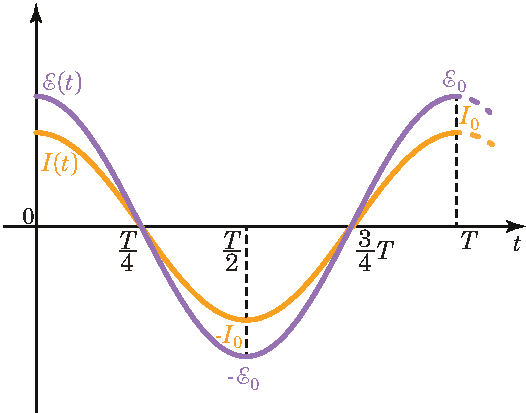
\includegraphics[width=0.5\textwidth]{images/chp11/chp11Rsymbgraf1.pdf}
\end{center}
Invece, se un resistore $R$ è attraversato da corrente alternata 
\begin{equation*}
	I(t)=I_0\cos(\omega t)
\end{equation*}
la \ddp ai capi è
\begin{equation}
	\tcboxmath[colback=yellowpastellow!30!white,drop fuzzy shadow, nobeforeafter, math upper, tcbox raise base, enhanced]{V_R(t)=RI(t)=RI_0\cos(\omega t)=V_{R,0}\cos(\omega t)}
\end{equation}
La \ddp e la corrente sono \textit{in fase} ($\oldphi_R=0$), con relazione tra i valori massimi dati da
\begin{equation}
	\tcboxmath[colback=yellowpastellow!30!white,drop fuzzy shadow, nobeforeafter, math upper, tcbox raise base, enhanced]{V_{R,0}=RI_0}
\end{equation}
\begin{center}
	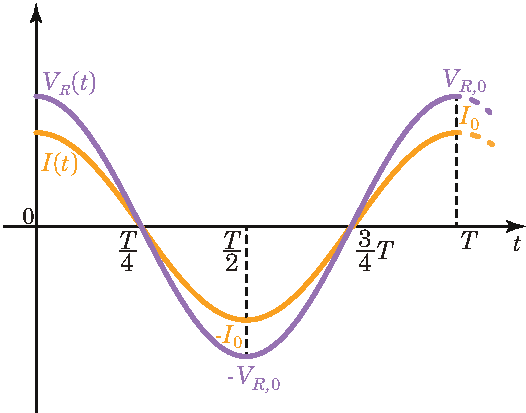
\includegraphics[width=0.5\textwidth]{images/chp11/chp11Rsymbgraf2.pdf}
\end{center}
\begin{observe}
	Il comportamento di un resistore in regime alternato \textit{non} dipende dal valore della pulsazione $\omega$.
\end{observe}
\paragraph{Metodo simbolico}
\begin{proposition}[Impedenza del resistore]
	L'impedenza di un resistore $R$ percorso da corrente alternata $I(t)=I_0\cos(\omega t)$ è
	\begin{equation}
		\tcboxmath[colback=yellowpastellow!30!white,colframe=orangered!85!black,drop fuzzy shadow, nobeforeafter, math upper, tcbox raise base, enhanced]{Z_R=R}
	\end{equation}
\end{proposition}
\begin{demonstrationopt}
	Definiamo il fasore della corrente elettrica
	\begin{equation*}
		\hat{I}(t)=I_0e^{i\omega t}=I_0\cos(\omega t)+iI_0\sin(\omega t)
	\end{equation*}
	e quello della \ddp ai capi del resistore $R$
	\begin{equation*}
		\hat{V}_R(t)=V_{R,0}e^{i(\omega t+\phi_R)}=V_{R,0}\cos(\omega t+\phi_R)+iV_{R,0}\sin(\omega t+\phi_R)
	\end{equation*}
	Dalla \textit{legge di Ohm} ricaviamo $\phi_R$ e $V_{R,0}$:
	\begin{equation*}
		V_R(t)=V_{R,0}\cos(\omega t+\phi_R)=RI_0\cos(\omega t)\implies \begin{cases}
			\phi_R=0\\
			V_{R,0}=R
		\end{cases} 
	\end{equation*}
	Di conseguenza, dalla definizione di impedenza segue
	\begin{equation*}
		Z_R=\frac{V_{R,0}}{I_0}e^{i\oldphi_R}=\frac{V_{R,0}}{I_0}=R\qedhere
	\end{equation*}
\end{demonstrationopt}
\subsection{Induttore L}
	\begin{center}		
	\begin{tikzpicture}
		\draw (0,0) to [sinusoidal current source, sV>=$\mathcal{E}(t)$] (0,2.5)
		-- (2.5,2.5)
		to [inductor, L=$L$, v=$V_L$] (2.5,0)
		-- (0,0)
		-- (0,0.1);
	\end{tikzpicture}
\end{center}
Applicando ai capi dell'induttore $R$ una \fem
\begin{equation*}
	\mathcal{E}(t)=\mathcal{E}_0\cos(\omega t)
\end{equation*}
la corrente che attraversa l'induttore è la soluzione all'equazione differenziale ordinaria
\begin{align*}
	&\mathcal{E}(t)-L\dv{I}{t}=0\\
	&\dv{I}{t}=\frac{\mathcal{E}(t)}{L}=\frac{\mathcal{E}_0}{L}\cos(\omega t)
\end{align*}
da cui otteniamo la legge
\begin{equation}
	\tcboxmath[colback=yellowpastellow!30!white,drop fuzzy shadow, nobeforeafter, math upper, tcbox raise base, enhanced]{I(t)=\frac{\mathcal{E}_0}{\omega L}\sin(\omega t)=\frac{\mathcal{E}_0}{\omega L}\cos(\omega t-\frac{\pi}{2})}
\end{equation}
La \fem e la corrente \textit{non} sono in fase, bensì sono sfasate di un fattore $\psi_L=-\nicefrac{\pi}{2}$.
\begin{center}
	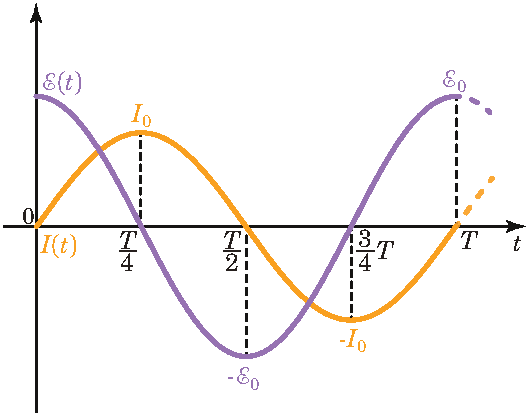
\includegraphics[width=0.5\textwidth]{images/chp11/chp11Lsymbgraf1.pdf}
\end{center}
Invece, se un resistore $R$ è attraversato da corrente alternata 
\begin{equation*}
	I(t)=I_0\cos(\omega t)
\end{equation*}
la \ddp ai capi è
\begin{equation}
	\tcboxmath[colback=yellowpastellow!30!white,drop fuzzy shadow, nobeforeafter, math upper, tcbox raise base, enhanced]{V_L(t)=L\dv{I(t)}{t}=-\omega L I_0\sin(\omega t)=V_{L,0}\cos(\omega t+\frac{\pi}{2})}
\end{equation}
La \ddp e la corrente \textit{non} sono in fase, bensì sono sfasate di un fattore $\oldphi_L=\nicefrac{\pi}{2}$.
\begin{center}
	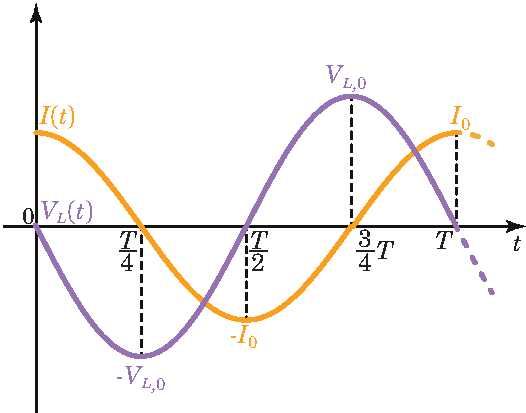
\includegraphics[width=0.5\textwidth]{images/chp11/chp11Lsymbgraf2.pdf}
\end{center}
\paragraph{Metodo simbolico}
\begin{proposition}[Impedenza dell'induttore]
	L'impedenza di un induttore $L$ percorso da corrente alternata $I(t)=I_0\cos\omega t$ è
	\begin{equation}
		\tcboxmath[colback=yellowpastellow!30!white,colframe=orangered!85!black,drop fuzzy shadow, nobeforeafter, math upper, tcbox raise base, enhanced]{Z_L=i\omega L}
	\end{equation}
\end{proposition}
\begin{demonstrationopt}
	Definiamo il fasore della corrente elettrica
	\begin{equation*}
		\hat{I}(t)=I_0e^{i\omega t}=I_0\cos(\omega t)+iI_0\sin(\omega t)
	\end{equation*}
	e quello della \ddp ai capi dell'induttore $L$
	\begin{equation*}
		\hat{V}_L(t)=V_{L,0}e^{i(\omega t+\phi_L)}=V_{L,0}\cos(\omega t+\phi_L)+iV_{L,0}\sin(\omega t+\phi_L)
	\end{equation*}
	Dalla relazione
	\begin{equation*}
		V_L(t)=L\dv{I}(t)
	\end{equation*}
	ricaviamo $\phi_L$ e $V_{L,0}$:
	\begin{equation*}
		V_L(t)=V_{L,0}\cos(\omega t+\phi_L)=-\omega L I_0\sin(\omega t)=\omega L I_0\cos(\omega t+\frac{\pi}{2})\implies \begin{cases}
			\phi_L=\frac{\pi}{2}\\
			V_{L,0}=\omega L I_0
		\end{cases} 
	\end{equation*}
	Di conseguenza, dalla definizione di impedenza segue
	\begin{equation*}
		Z_L=\frac{V_{L,0}}{I_0}e^{i\oldphi_L}=\omega Le^{i\frac{\pi}{2}}=i\omega L\qedhere
	\end{equation*}
\end{demonstrationopt}
\subsection{Condensatore C}
	\begin{center}		
	\begin{tikzpicture}
		\draw (0,0) to [sinusoidal current source, v<=$\mathcal{E}(t)$] (0,2.5)
		-- (2.5,2.5)
		to [capacitor, C=$C$, v=$V_C$] (2.5,0)
		-- (0,0)
		-- (0,0.1);
	\end{tikzpicture}
\end{center}
Applicando ai capi del condensatore $C$ una \fem
\begin{equation*}
	\mathcal{E}(t)=\mathcal{E}_0\cos(\omega t)
\end{equation*}
la carica che si deposita sulle armature del condensatore è data da
\begin{equation*}
	\mathcal{E}(t)=V_C(t)=\frac{q(t)}{C}
\end{equation*}
\begin{equation}
		\tcboxmath[colback=yellowpastellow!30!white,drop fuzzy shadow, nobeforeafter, math upper, tcbox raise base, enhanced]{q(t)=C\mathcal{E}(t)=C\mathcal{E}_0\cos(\omega t)}
\end{equation}
La corrente che attraversa l'induttore si ottiene derivando la precedente relazione
\begin{equation*}
	I(t)=\dv{q(t)}{T}=C\dv{\mathcal{E}(t)}{t}\\
\end{equation*}
da cui otteniamo la legge
\begin{equation}
		\tcboxmath[colback=yellowpastellow!30!white,drop fuzzy shadow, nobeforeafter, math upper, tcbox raise base, enhanced]{I(t)=\mathcal{E}_0\omega C\sin(\omega t)=\mathcal{E}_0\omega C\cos(\omega t+\frac{\pi}{2})}
\end{equation}
La \fem e la corrente \textit{non} sono in fase, bensì sono sfasate di un fattore $\psi_C=\nicefrac{\pi}{2}$.
\begin{center}
	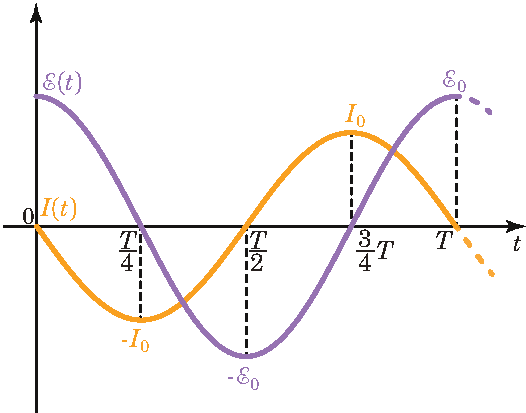
\includegraphics[width=0.5\textwidth]{images/chp11/chp11Csymbgraf1.pdf}
\end{center}
Invece, se un resistore $R$ è attraversato da corrente alternata
\begin{equation*}
	I(t)=I_0\cos(\omega t)
\end{equation*}
la \ddp ai capi è data dalla legge
\begin{equation*}
	V_C(t)=\frac{q(t)}{C}
\end{equation*}
o, equivalentemente, integrando la seguente:
\begin{equation*}
	\dv{V_C(t)}{t}=\frac{1}{C}dv{q(t)}{t}=\frac{I(t)}{C}=\frac{I_0}{C}\cos(\omega t)
\end{equation*}
\begin{equation}
		\tcboxmath[colback=yellowpastellow!30!white,drop fuzzy shadow, nobeforeafter, math upper, tcbox raise base, enhanced]{V_C(t)=\frac{I_0}{\omega C}\sin(\omega t)=\frac{I_0}{\omega C}\cos(\omega t-\frac{\pi}{2})=V_{C,0}\cos(\omega t-\frac{\pi}{2})}
\end{equation}
La \ddp e la corrente \textit{non} sono in fase, bensì sono sfasate di un fattore $\oldphi_C=-\nicefrac{\pi}{2}$.
\begin{center}
	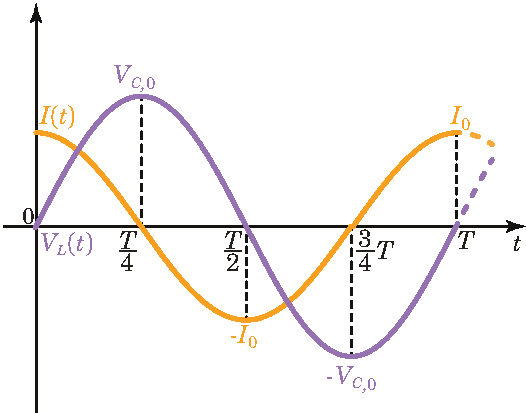
\includegraphics[width=0.5\textwidth]{images/chp11/chp11Csymbgraf2.pdf}
\end{center}
\paragraph{Metodo simbolico}
\begin{proposition}[Impedenza del condensatore]
	L'impedenza di un condensatore $L$ percorso da corrente alternata $I(t)=I_0\cos\omega t$ è
	\begin{equation}
		\tcboxmath[colback=yellowpastellow!30!white,colframe=orangered!85!black,drop fuzzy shadow, nobeforeafter, math upper, tcbox raise base, enhanced]{Z_C=\frac{1}{i \omega C}}
	\end{equation}
\end{proposition}
\begin{demonstrationopt}
	Definiamo il fasore della corrente elettrica
	\begin{equation*}
		\hat{I}(t)=I_0e^{i\omega t}=I_0\cos(\omega t)+iI_0\sin(\omega t)
	\end{equation*}
	e quello della \ddp ai capi del condensatore $C$
	\begin{equation*}
		\hat{V}_C(t)=V_{C,0}e^{i(\omega t+\phi_C)}=V_{C,0}\cos(\omega t+\phi_C)+iV_{C,0}\sin(\omega t+\phi_C)
	\end{equation*}
	Integrando
	\begin{equation*}
		\dv{V_C(t)}{t}=\frac{1}{C}dv{q(t)}{t}=\frac{I(t)}{C}=\frac{I_0}{C}\cos(\omega t)
	\end{equation*}
	ricaviamo $\phi_C$ e $V_{C,0}$:
	\begin{equation*}
		V_C(t)=V_{C,0}\cos(\omega t+\phi_C)=\frac{I_0}{\omega C}\sin(\omega t)=\frac{I_0}{\omega C}\cos(\omega t-\frac{\pi}{2})\implies \begin{cases}
			\phi_C=-\frac{\pi}{2}\\
			V_{C,0}=\frac{I_0}{\omega C}
		\end{cases} 
	\end{equation*}
	Di conseguenza, dalla definizione di impedenza segue
	\begin{equation*}
		Z_C=\frac{V_{C,0}}{I_0}e^{i\oldphi_C}=\frac{1}{\omega C}e^{-i\frac{\pi}{2}}=\frac{1}{i \omega C}\qedhere
	\end{equation*}
\end{demonstrationopt}
\subsection{Circuito RL in serie}
	\begin{center}		
	\begin{tikzpicture}
		\draw (0,0) to [sinusoidal current source, v<=$\mathcal{E}(t)$] (0,2.5)
		to [resistor, R=$R$, v=$V_R$] (2.5,2.5)
		to [inductor, L=$L$, v=$V_L$] (2.5,0)
		-- (0,0)
		-- (0,0.1);
	\end{tikzpicture}
\end{center}
Se nel circuito circola una corrente alternata di intensità
\begin{equation*}
	I(t)=I_0\cos(\omega t)
\end{equation*}
le differenze ai capi del resistore e dell'induttore sono
\begin{align*}
	V_R(t)&=V_{R,0}\cos(\omega t +\oldphi_R)=\abs{Z_R}I_0\cos(\omega t +\oldphi_R)=RI_0\cos(\omega t)
	\\
	V_L(t)&=V_{L,0}\cos(\omega t +\oldphi_L)=\abs{Z_L}I_0\cos(\omega t +\oldphi_L)=\omega LI_0\cos(\omega t +\frac{\pi}{2})
\end{align*}
L'impedenza complessiva è la somma delle impedenze dei singoli componenti:
\begin{align}
	Z_{RL}&=Z_R+Z_L=R+i\omega L\\
	\abs{Z_{RL}}&=\sqrt{R^2+\omega^2L^2}
\end{align}
La \ddp complessiva è data dalla somma di $V_R(t)$ e $V_L(t)$, che possiamo ottenere sia come somma di fasori, sia tramite la rappresentazione vettoriale.
\begin{equation*}
	V(t)=V_R(t)+V_L(t)=V_{RL,0}\cos(\omega t+\oldphi_{RL})
\end{equation*}
dove
\begin{align*}
	V_{RL,0}&=\sqrt{V_{R,0}^2+V_{L,0}^2+V_{R,0}V_{L,0}\cos(\oldphi_R-\oldphi_L)}=\\
	&=\sqrt{(RI_0)^2+(\omega LI_0)^2+\Ccancel[red]{2(RI_0)(\omega LI_0)\cos(0-\frac{\pi}{2})}}=\\
	&=\sqrt{R^2+\omega^2L^2}I_0=\sqrt{Z_R^2+Z_L^2}I_0=\abs{Z_{RL}}I_0
\end{align*}
\begin{equation*}
	\tan\oldphi_{RL}=\frac{V_{R,0}\sin\oldphi_R+V_{L,0}\sin\oldphi_L}{V_{R,0}\cos\oldphi_R+V_{L,0}\cos\oldphi_L}=\frac{RI_0\sin0+\omega LI_0\sin\frac{\pi}{2}}{RI_0\cos0+\omega LI_0\cos\frac{\pi}{2}}=\frac{\omega L\Ccancel[red]{I_0}}{R\Ccancel[red]{I_0}}=\frac{\abs{Z_L}}{\abs{Z_R}}
\end{equation*}
\begin{center}
	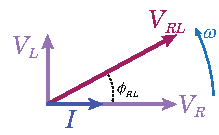
\includegraphics[width=0.35\textwidth]{images/chp11/chp11fasoriRL.pdf}
\end{center}
\subsection{Circuito RC in serie}
	\begin{center}		
	\begin{tikzpicture}
		\draw (0,0) to [sinusoidal current source, v<=$\mathcal{E}(t)$] (0,2.5)
		to [resistor, R=$R$, v=$V_R$] (2.5,2.5)
		to [capacitor, C=$C$, v=$V_C$] (2.5,0)
		-- (0,0)
		-- (0,0.1);
	\end{tikzpicture}
\end{center}
Se nel circuito circola una corrente alternata di intensità
\begin{equation*}
	I(t)=I_0\cos(\omega t)
\end{equation*}
le differenze ai capi del resistore e del condensatore sono
\begin{align*}
	V_R(t)&=V_{R,0}\cos(\omega t +\oldphi_R)=\abs{Z_R}I_0\cos(\omega t +\oldphi_R)=RI_0\cos(\omega t)\\
	V_C(t)&=V_{C,0}\cos(\omega t +\oldphi_C)=\abs{Z_C}I_0\cos(\omega t +\oldphi_C)=\frac{I_0}{\omega C}\cos(\omega t -\frac{\pi}{2})
\end{align*}
L'impedenza complessiva è la somma delle impedenze dei singoli componenti:
\begin{empheq}[box=\tcmathboxgeneral]{align}
	Z_{RL}&=Z_R+Z_C=R+\frac{1}{i\omega C}=R-i\frac{1}{\omega C}\\ \abs{Z_{RC}}&=\sqrt{R^2+\frac{1}{\omega^2 C^2}}
\end{empheq}
La \ddp complessiva è data dalla somma di $V_R(t)$ e $V_C(t)$, che possiamo ottenere sia come somma di fasori, sia tramite la rappresentazione vettoriale.
\begin{equation*}
	V(t)=V_R(t)+V_C(t)=V_{RC,0}\cos(\omega t+\oldphi_{RC})
\end{equation*}
dove
\begin{align*}
	V_{RC,0}&=\sqrt{V_{R,0}^2+V_{C,0}^2+V_{R,0}V_{C,0}\cos(\oldphi_R-\oldphi_C)}=\\
	&=\sqrt{(RI_0)^2+(\frac{I_0}{i\omega C})^2+\Ccancel[red]{2(RI_0)(\frac{I_0}{i\omega C})\cos(0+\frac{\pi}{2})}}=\\
	&=\sqrt{R^2+\frac{1}{\omega^2 C^2}}I_0=\sqrt{Z_R^2+Z_C^2}I_0=\abs{Z_{RC}}I_0
\end{align*}
\begin{equation*}
	\tan\oldphi_{RC}=\frac{V_{R,0}\sin\oldphi_R+V_{C,0}\sin\oldphi_C}{V_{R,0}\cos\oldphi_R+V_{C,0}\cos\oldphi_C}=\frac{RI_0\sin0+\frac{I_0}{\omega C}\sin\left(-\frac{\pi}{2}\right)}{RI_0\cos0+\frac{I_0}{\omega C}\cos\left(-\frac{\pi}{2}\right)}=\frac{\frac{\Ccancel[red]{I_0}}{\omega C}}{R\Ccancel[red]{I_0}}=\frac{1}{\omega RC}=-\frac{\abs{Z_C}}{\abs{Z_R}}
\end{equation*}
\begin{center}
	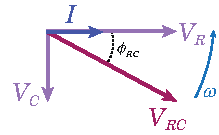
\includegraphics[width=0.35\textwidth]{images/chp11/chp11fasoriRC.pdf}
\end{center}
\subsection{Circuito LC in serie}
	\begin{center}		
	\begin{tikzpicture}
		\draw (0,0) to [sinusoidal current source, V_=$\mathcal{E}(t)$] (0,2.5)
		to [inductor, L=$L$, v=$V_L$] (2.5,2.5)
		to [capacitor, C=$C$, v=$V_C$] (2.5,0)
		-- (0,0)
		-- (0,0.1);
	\end{tikzpicture}
\end{center}
Se nel circuito circola una corrente alternata di intensità
\begin{equation*}
	I(t)=I_0\cos(\omega t)
\end{equation*}
le differenze ai capi dell'induttore e del condensatore sono
\begin{align*}
	V_L(t)&=V_{L,0}\cos(\omega t +\oldphi_L)=\abs{Z_L}I_0\cos(\omega t +\oldphi_L)=\omega L I_0\cos(\omega t+\frac{\pi}{2})
	\\
	V_C(t)&=V_{C,0}\cos(\omega t +\oldphi_C)=\abs{Z_C}I_0\cos(\omega t +\oldphi_C)=\frac{I_0}{\omega C}\cos(\omega t -\frac{\pi}{2})
\end{align*}
L'impedenza complessiva è la somma delle impedenze dei singoli componenti:
\begin{empheq}[box=\tcmathboxgeneral]{align}
	Z_{LC}&=Z_L+Z_C=i\omega L+\frac{1}{i\omega C}=i\left(\omega L-\frac{1}{\omega C}\right)\\
\abs{Z_{LC}}&=\abs{\omega L-\frac{1}{\omega C}}
\end{empheq}
La \ddp complessiva è data dalla somma di $V_L(t)$ e $V_C(t)$, che possiamo ottenere sia come somma di fasori, sia tramite la rappresentazione vettoriale.
\begin{equation*}
	V(t)=V_L(t)+V_C(t)=V_{LC,0}\cos(\omega t+\oldphi_{LC})
\end{equation*}
dove
\begin{align*}
	V_{LC,0}&=\sqrt{V_{L,0}^2+V_{C,0}^2+V_{L,0}V_{C,0}\cos(\oldphi_L-\oldphi_C)}=\\
	&=\sqrt{(\omega L I_0)^2+(\frac{I_0}{\omega C})^2+2(\omega L I_0)(\frac{I_0}{\omega C})\cos(\frac{\pi}{2}+\frac{\pi}{2})}=\\
	&=\sqrt{(\omega L I_0)^2+(\frac{I_0}{\omega C})^2-2(\omega L I_0)(\frac{I_0}{\omega C})}I_0=\abs{\omega L I_0-\frac{I_0}{\omega C}}I_0=\\
	&=\abs{Z_L-Z_C}I_0=\abs{Z_{LC}}I_0
\end{align*}
\begin{align*}
	\oldphi_{LC}&=\mathrm{sgn}\left(V_{L,0}\cos\oldphi_L+V_{C,0}\cos\oldphi_C\right)\frac{\pi}{2}=\mathrm{sgn}\left(\omega L I_0\sin\frac{\pi}{2}+\frac{I_0}{\omega C}\sin\left(-\frac{\pi}{2}\right)\right)\frac{\pi}{2}=\\
	&=\mathrm{sgn}\left(\omega L I_0-\frac{I_0}{\omega C}\right)\frac{\pi}{2}=\mathrm{sgn}\left(\omega L -\frac{1}{\omega C}\right)\frac{\pi}{2}=\mathrm{sgn}\left(Z_L - Z_C\right)\frac{\pi}{2}=\\
	&=\begin{cases}
		\frac{\pi}{2}&Z_L>Z_C\\
		-\frac{\pi}{2}&Z_L<Z_C\\
	\end{cases}
\end{align*}
\begin{minipage}{0.49\textwidth}
	\begin{center}
		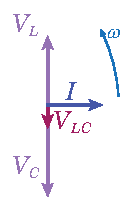
\includegraphics[width=0.45\textwidth]{images/chp11/chp11fasoriLC2.pdf}
	\end{center}
$$\omega L<\frac{1}{\omega C}$$
\end{minipage}
\begin{minipage}{0.49\textwidth}
	\begin{center}
		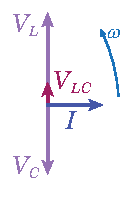
\includegraphics[width=0.45\textwidth]{images/chp11/chp11fasoriLC1.pdf}
		$$\omega L>\frac{1}{\omega C}$$
	\end{center}
\end{minipage}
\subsection{Circuito RLC in serie}
\begin{center}
	\begin{tikzpicture}[voltage dir=RP]
		\draw (0,0) to [sinusoidal current source, V_=$\mathcal{E}(t)$] (0,2.5)
		to [resistor, R=$R$, v=$V_R$] (2.5,2.5)
		to [inductor, L=$L$, v=$V_L$] (2.5,0)
		to [capacitor, C=$C$, v=$V_C$] (0,0)
		-- (0,0.1);
	\end{tikzpicture}
\end{center}
Se nel circuito circola una corrente alternata di intensità
\begin{equation*}
	I(t)=I_0\cos(\omega t)
\end{equation*}
le differenze ai capi dei componenti elettrici sono
\begin{align*}
	V_R(t)&=V_{R,0}\cos(\omega t +\oldphi_R)=\abs{Z_R}I_0\cos(\omega t +\oldphi_R)=RI_0\cos(\omega t)\\
	V_L(t)&=V_{L,0}\cos(\omega t +\oldphi_L)=\abs{Z_L}I_0\cos(\omega t +\oldphi_L)=\omega L I_0\cos(\omega t+\frac{\pi}{2})
	\\
	V_C(t)&=V_{C,0}\cos(\omega t +\oldphi_C)=\abs{Z_C}I_0\cos(\omega t +\oldphi_C)=\frac{I_0}{\omega C}\cos(\omega t -\frac{\pi}{2})
\end{align*}
L'impedenza complessiva è la somma delle impedenze dei singoli componenti:
\begin{empheq}[box=\tcmathboxgeneral]{align}
	Z_{RLC}&=Z_R+Z_L+Z_C=R+i\omega L+\frac{1}{i\omega C}=R+i\left(\omega L-\frac{1}{\omega C}\right)\\
\abs{Z_{RLC}}&=\sqrt{R^2+\left(\omega L-\frac{1}{\omega C}\right)^2}
\end{empheq}
In forma esponenziale, essa è
\begin{equation*}
	Z_{RLC}=\abs{Z_{RLC}}e^{i\oldphi_{RLC}}
\end{equation*}
dove
\begin{equation*}
	\tan\oldphi_{RLC}=\frac{\Im Z_{RLC}}{\Re Z_{RLC}}=\frac{\omega L -\frac{1}{\omega C}}{R}
\end{equation*}
Presa la corrente complessa
\begin{equation*}
	\hat{I}(t)=I_0e^{i\omega t}
\end{equation*}
la \ddp complessa totale risulta
\begin{equation*}
	\hat{V}(t)=Z_{RLC}\hat{I}(t)=\abs{Z_{RLC}}I_0e^{i\omega t}e^{i\theta}=\sqrt{R^2+\left(\omega L-\frac{1}{\omega C}\right)^2}I_0e^{i\omega t}e^{i\theta}
\end{equation*}
In termini non complessi il voltaggio è pari a
\begin{equation*}
	V(t)=\sqrt{R^2+\left(\omega L-\frac{1}{\omega C}\right)^2}I_0\cos(\omega t +\theta)
\end{equation*}
\begin{minipage}{0.33\textwidth}
	\begin{center}
		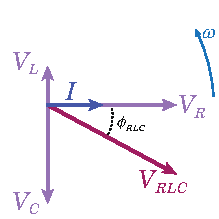
\includegraphics[width=0.9\textwidth]{images/chp11/chp11fasoriRLC2.pdf}
		$\omega L<\frac{1}{\omega C}$
	\end{center}
\end{minipage}
\begin{minipage}{0.33\textwidth}
	\begin{center}
		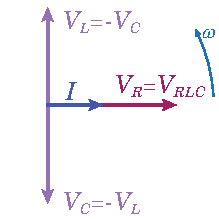
\includegraphics[width=0.9\textwidth]{images/chp11/chp11fasoriRLC3.pdf}
		$\omega L=\frac{1}{\omega C}$
	\end{center}
\end{minipage}
\begin{minipage}{0.33\textwidth}
	\begin{center}
		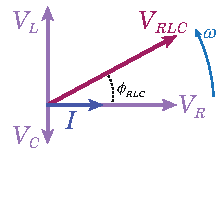
\includegraphics[width=0.9\textwidth]{images/chp11/chp11fasoriRLC1.pdf}
		$\omega L>\frac{1}{\omega C}$
	\end{center}
\end{minipage}
\subsubsection{Selezionatore di frequenze}
La relazione tra la corrente massima $I_0$ e la \ddp massima $V_0$ c'è la relazione
\begin{equation}\label{relazioneACmaxmin}
	\tcboxmath[colback=yellowpastellow!30!white,drop fuzzy shadow, nobeforeafter, math upper, tcbox raise base, enhanced]{I_0=\frac{V_0}{Z_0}=\frac{V_0}{\sqrt{R^2+\left(\omega L -\frac{1}{\omega C}\right)^2}}}
\end{equation}
Fissata la differenza di potenziale $V_0$ ai capi delle componenti e i loro valori $L$, $C$ ed $R$, la corrente $I_0$ risulta dipendere esclusivamente dalla pulsazione $\omega$ - a cui corrisponde una particolare frequenza $\nu$ tale per cui
\begin{equation}
	\tcboxmath[colback=yellowpastellow!30!white,drop fuzzy shadow, nobeforeafter, math upper, tcbox raise base, enhanced]{\omega=2\pi \nu}
\end{equation}
Fra tutte le frequenze ammissibili, ce n'è una di particolare rilevanza.
\begin{define}[Frequenza di risonanza]
	La \textbf{frequenza di risonanza}\index{frequenza!di risonanza} di un circuito AC in serie è la frequenza tale per cui l'impedenza del circuito è minima e la fase è nulla.
\end{define}
Dalla \eqref{relazioneACmaxmin} è evidente che minore è l'impedenza, maggiore sarà la corrente che scorre nel circuito.
\begin{center}
	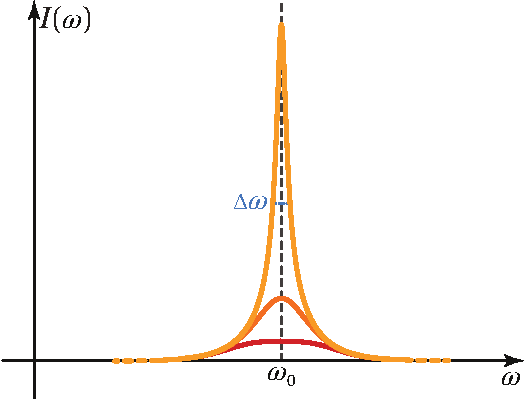
\includegraphics[width=0.7\textwidth]{images/chp11/chp11correnterisonanzagraf.pdf}
\end{center}
Nel caso del circuito $RLC$ in serie, osserviamo come dal punto di vista fasoriale le impedenze $Z_L$ e $Z_C$ hanno la stessa direzione, ma versi opposti e moduli che dipendono dalla frequenza, mentre l'impedenza del resistore $Z_R$ \textit{non} dipende dalla frequenza ed è ortogonale alle altre. Di conseguenza, è immediato realizzare che la \textit{condizione di risonanza} si ha quando la \textit{reattanza} è nulla.
\begin{equation*}
	0=X_{RLC}=\Im Z_{RLC}=\omega_0 L-\frac{1}{\omega_0 C}
\end{equation*}
da cui segue che
\begin{equation*}
	\omega_0=\frac{1}{\sqrt{LC}}
\end{equation*}
I circuiti risonanti sono utilizzati per rispondere \textit{selettivamente} a segnali di una certa frequenza, trascurando segnali di frequenze diverse: scelta la frequenza di risonanza $\omega_0$, l'intensità di corrente che scorre nel circuito presenta un picco in sua corrispondenza.

Se consideriamo la larghezza $\Delta \omega$ della \textit{curva di risonanza} - ossia del grafico $\omega-I$ - a metà del massimo, possiamo introdurre un \textbf{fattore di qualità}\index{fattore di qualità}
\begin{equation}
	\tcboxmath[colback=yellowpastellow!30!white,drop fuzzy shadow, nobeforeafter, math upper, tcbox raise base, enhanced]{Q=\frac{\omega_0}{\Delta \omega}}
\end{equation}
Maggiore è $Q$, più evidente sarà il massimo assunto dalla corrente e minore la corrente che scorre nel circuito a frequenze differenti. Si può osservare che
\begin{equation}
	\tcboxmath[colback=yellowpastellow!30!white,drop fuzzy shadow, nobeforeafter, math upper, tcbox raise base, enhanced]{\Delta \omega\sim \frac{R}{L}}
\end{equation}
Facendo tendere $\nicefrac{R}{L}$ a zero segue che anche $\Delta \omega$ tende a zero e quindi il fattore $Q$ diventa molto elevato: la curva di risonanza risulta essere praticamente nulla per tutte le frequenze eccetto quella di risonanza. Di conseguenza, di fatto \textit{non scorre corrente nel circuito} a meno di essere in presenza della frequenza di risonanza.

Quello che abbiamo descritto è sostanzialmente il funzionamento dei radioricevitori per le \textit{radio AM}: la selettività della sintonizzazione deve essere tale da escludere le stazioni radio sopra e sotto la \textit{frequenza portante} - quella che vogliamo ascoltare -  ma non così elevata da escludere le \textit{bande laterali}, causate dalla modulazione d'ampiezza del segnale.
%TODO:grafico?
\subsection{⋆ Circuito RL in parallelo}
\begin{center}		
	\begin{tikzpicture}[voltage dir=RP]
		\draw (5,0) -- (0,0)
					to [sinusoidal current source, V_=$\mathcal{E}(t)$] (0,2.5)
					-- (5,2.5);
		\draw (2.5,2.5) to [resistor, R=$R$, v=$V_R$] 	(2.5,0);
		\draw (5,2.5) 	to [inductor, L=$L$, v=$V_L$] 	(5,0);
	\end{tikzpicture}
\end{center}
Se ai capi dei rami i paralleli c'è una \ddp alternata
\begin{equation*}
	V(t)=V_0\cos(\omega t)
\end{equation*}
le correnti che attraversano il resistore e l'induttore sono
\begin{align*}
	I_R(t)&=I_{R,0}\cos(\omega t +\oldphi_R)=\frac{V_0}{\abs{Z_R}}\cos(\omega t +\oldphi_R)=\frac{V_0}{R}\cos(\omega t)\\
	I_L(t)&=I_{L,0}\cos(\omega t +\oldphi_L)=\frac{V_0}{\abs{Z_L}}\cos(\omega t +\oldphi_L)=\frac{V_0}{\omega L}\cos(\omega t -\frac{\pi}{2})
\end{align*}
L'ammettenza complessiva è la somma delle ammettenze dei singoli componenti:
\begin{align*}
	\frac{1}{Z_{RL}}&=\frac{1}{Z_R}+\frac{1}{Z_L}=\frac{1}{R}+\frac{1}{i\omega L}=\frac{1}{R}-i\frac{1}{\omega L}\\
	Z_{RL}&=\frac{1}{\frac{1}{R}-i\frac{1}{\omega L}}=\frac{\omega L R}{\omega L-iR}=\frac{\omega^2 L^2 R}{R^2+\omega^2 L^2}+i\frac{\omega L R^2}{R^2+\omega^2 L^2}\\
	\abs{Z_{RL}}&=\sqrt{\frac{\omega^4 L^4 R^2+\omega^2 L^2 R^4}{\left(R^2+\omega^2 L^2\right)^2}}=\sqrt{\frac{\left(\omega^2 L^2 R^2\right)\Ccancel[red]{\left(R^2+\omega^2 L^2\right)}}{\left(R^2+\omega^2 L^2\right)^{\Ccancel[red]{2}}}}=\frac{\omega L R}{\sqrt{R^2+\omega^2L^2}}
\end{align*}
\begin{empheq}[box=\tcmathboxgeneral]{align}
	Z_{RL}&=\frac{\omega^2 L^2 R}{R^2+\omega^2 L^2}+i\frac{\omega L R^2}{R^2+\omega^2 L^2}\\
\abs{Z_{RL}}&=\frac{\omega L R}{\sqrt{R^2+\omega^2L^2}}
\end{empheq}
In forma esponenziale, essa è
\begin{equation*}
	Z_{RL}=\abs{Z_{RL}}e^{i\theta}
\end{equation*}
dove
\begin{equation*}
	\tan\theta=\frac{\Im Z_{RL}}{\Re Z_{RL}}=\frac{R}{\omega L}
\end{equation*}
Presa la \ddp complessa
\begin{equation*}
	\hat{V}(t)=V_0e^{i\omega t}
\end{equation*}
la corrente complessa totale risulta
\begin{equation*}
	\hat{I}(t)=\frac{1}{Z_{RL}}\hat{V}(t)=\frac{1}{\abs{Z_{RL}}}V_0e^{i\omega t}e^{-i\theta}=\frac{\sqrt{R^2+\omega^2L^2}}{\omega L R}V_0e^{i\omega t}e^{-i\theta}
\end{equation*}
In termini non complessi il voltaggio è pari a
\begin{equation*}
	V(t)=\frac{\sqrt{R^2+\omega^2L^2}}{\omega L R}V_0\cos(\omega t -\theta)
\end{equation*}
\subsection{⋆ Circuito RC in parallelo}
\begin{center}		
	\begin{tikzpicture}[voltage dir=RP]
		\draw (5,0) -- (0,0)
		to [sinusoidal current source, V_=$\mathcal{E}(t)$] (0,2.5)
		-- (5,2.5);
		\draw (2.5,2.5) to [resistor, R=$R$, v=$V_R$] 	(2.5,0);
		\draw (5,2.5) 	to [capacitor, C=$C$, v=$V_C$] 	(5,0);
	\end{tikzpicture}
\end{center}
Se ai capi dei rami i paralleli c'è una \ddp alternata
\begin{equation*}
	V(t)=V_0\cos(\omega t)
\end{equation*}
le correnti che attraversano il resistore e l'induttore sono
\begin{align*}
	I_R(t)&=I_{R,0}\cos(\omega t +\oldphi_R)=\frac{V_0}{\abs{Z_R}}\cos(\omega t +\oldphi_R)=\frac{V_0}{R}\cos(\omega t)\\
	I_C(t)&=I_{C,0}\cos(\omega t +\oldphi_C)=\frac{V_0}{\abs{Z_C}}\cos(\omega t +\oldphi_C)=\omega C V_0\cos(\omega t +\frac{\pi}{2})
\end{align*}
L'ammettenza complessiva è la somma delle ammettenze dei singoli componenti:
\begin{align*}
	\frac{1}{Z_{RC}}&=\frac{1}{Z_R}+\frac{1}{Z_C}=\frac{1}{R}+i\omega C\\
	Z_{RC}&=\frac{1}{\frac{1}{R}+i\omega C}=\frac{R}{1+i\omega C R}=\frac{R}{1+\omega^2 C^2 R^2}-i\frac{\omega C R^2}{1+\omega^2 C^2 R^2}\\
	\abs{Z_{RL}}&=\sqrt{\frac{R^2+\omega^2 C^2 R^4}{\left(1+\omega^2 C^2 R^2\right)^2}}=\sqrt{\frac{R^2\Ccancel[red]{\left(1+\omega^2 C^2 R^2\right)}}{\left(1+\omega^2 C^2 R^2\right)^{\Ccancel[red]{2}}}}=\frac{R}{\sqrt{1+\omega^2 C^2 R^2}}
\end{align*}
\begin{empheq}[box=\tcmathboxgeneral]{align}
	Z_{RC}&=\frac{R}{1+\omega^2 C^2 R^2}-i\frac{\omega C R^2}{1+\omega^2 C^2 R^2} \\
\abs{Z_{RC}}&=\frac{R}{\sqrt{1+\omega^2 C^2 R^2}}
\end{empheq}
In forma esponenziale, essa è
\begin{equation*}
	Z_{RC}=\abs{Z_{RC}}e^{i\theta}
\end{equation*}
dove
\begin{equation*}
	\tan\theta=\frac{\Im Z_{RC}}{\Re Z_{RC}}=-\omega C R
\end{equation*}
Presa la \ddp complessa
\begin{equation*}
	\hat{V}(t)=V_0e^{i\omega t}
\end{equation*}
la corrente complessa totale risulta
\begin{equation*}
	\hat{I}(t)=\frac{1}{Z_{RC}}\hat{V}(t)=\frac{1}{\abs{Z_{RC}}}V_0e^{i\omega t}e^{-i\theta}=\frac{\sqrt{1+\omega^2 C^2 R^2}}{R}V_0e^{i\omega t}e^{-i\theta}
\end{equation*}
In termini non complessi il voltaggio è pari a
\begin{equation*}
	V(t)=\frac{\sqrt{1+\omega^2 C^2 R^2}}{R}V_0\cos(\omega t -\theta)
\end{equation*}
\subsection{⋆ Circuito LC in parallelo}
\begin{center}		
	\begin{tikzpicture}[voltage dir=RP]
		\draw (5,0) -- (0,0)
		to [sinusoidal current source, V_=$\mathcal{E}(t)$] (0,2.5)
		-- (5,2.5);
		\draw (2.5,2.5) 	to [inductor, L=$L$, v=$V_L$] 	(2.5,0);
		\draw (5,2.5) 	to [capacitor, C=$C$, v=$V_C$] 	(5,0);
	\end{tikzpicture}
\end{center}
Se ai capi dei rami i paralleli c'è una \ddp alternata
\begin{equation*}
	V(t)=V_0\cos(\omega t)
\end{equation*}
le correnti che attraversano il resistore e l'induttore sono
\begin{align*}
	I_L(t)&=I_{L,0}\cos(\omega t +\oldphi_L)=\frac{V_0}{\abs{Z_L}}\cos(\omega t +\oldphi_L)=\frac{V_0}{\omega L}\cos(\omega t -\frac{\pi}{2})\\
	I_C(t)&=I_{C,0}\cos(\omega t +\oldphi_C)=\frac{V_0}{\abs{Z_C}}\cos(\omega t +\oldphi_C)=\omega C V_0\cos(\omega t +\frac{\pi}{2})
\end{align*}
L'ammettenza complessiva è la somma delle ammettenze dei singoli componenti:
\begin{align*}
	\frac{1}{Z_{LC}}&=\frac{1}{Z_L}+\frac{1}{Z_C}=\frac{1}{i\omega L}+i\omega C=i\left(\omega C-\frac{1}{\omega L}\right)\\
	Z_{RC}&=\frac{1}{i\left(\omega C-\frac{1}{\omega L}\right)}=-i\frac{\omega L}{\omega^2 L C - 1}\\
	\abs{Z_{LC}}&=\abs{\frac{\omega L}{\omega^2 L C - 1}}=\frac{\omega L}{\abs{\omega^2 L C - 1}}
\end{align*}
\begin{empheq}[box=\tcmathboxgeneral]{align}
	Z_{LC}&=-i\frac{\omega L}{\omega^2 L C - 1} \\
\abs{Z_{LC}}&=\frac{\omega L}{\abs{\omega^2 L C - 1}}
\end{empheq}
In forma esponenziale, essa è
\begin{equation*}
	Z_{LC}=\abs{Z_{LC}}e^{i\theta}
\end{equation*}
dove
\begin{align*}
	\theta&=\mathrm{sgn}\left(1-\omega^2 L C\right)\frac{\pi}{2}=\mathrm{sgn}\left(\frac{1}{\omega L} - \omega C\right)\frac{\pi}{2}=\mathrm{sgn}\left(\frac{1}{\abs{Z_L}} - \frac{1}{\abs{Z_C}}\right)\frac{\pi}{2}=\\
	&=\begin{cases}
		\frac{\pi}{2}&Z_C>Z_L\\
		-\frac{\pi}{2}&Z_C<Z_L	
	\end{cases}
\end{align*}
\begin{observe}
	Per $Z_C=Z_L$, ossia se $\omega$ coincide con la frequenza di risonanza, l'impedenza è nulla e la corrente si annulla, essendo $I_L=-I_C$.
\end{observe}
Presa la \ddp complessa
\begin{equation*}
	\hat{V}(t)=V_0e^{i\omega t}
\end{equation*}
la corrente complessa totale risulta
\begin{equation*}
	\hat{I}(t)=\frac{1}{Z_{LC}}\hat{V}(t)=\frac{1}{\abs{Z_{LC}}}V_0e^{i\omega t}e^{-i\theta}=\frac{\abs{\omega^2 L C - 1}}{\omega L}V_0e^{i\omega t}e^{-i\theta}
\end{equation*}
In termini non complessi il voltaggio è pari a
\begin{equation*}
	V(t)=\frac{\abs{\omega^2 L C - 1}}{\omega L}V_0\cos(\omega t -\theta)
\end{equation*}
\subsection{⋆ Circuito  RLC in parallelo}
\begin{center}		
	\begin{tikzpicture}[voltage dir=RP]
		\draw (7.5,0) -- (0,0)
		to [sinusoidal current source, V_=$\mathcal{E}(t)$] (0,2.5)
		-- (7.5,2.5);
		\draw (2.5,2.5) to [resistor, R=$R$, v=$V_R$] 	(2.5,0);
		\draw (5,2.5) 	to [inductor, L=$L$, v=$V_L$] 	(5,0);
		\draw (7.5,2.5) 	to [capacitor, C=$C$, v=$V_C$] 	(7.5,0);
	\end{tikzpicture}
\end{center}
Se ai capi dei rami i paralleli c'è una \ddp alternata
\begin{equation*}
	V(t)=V_0\cos(\omega t)
\end{equation*}
le correnti che attraversano il resistore e l'induttore sono
\begin{align*}
	I_R(t)&=I_{R,0}\cos(\omega t +\oldphi_R)=\frac{V_0}{\abs{Z_R}}\cos(\omega t +\oldphi_R)=\frac{V_0}{R}\cos(\omega t)\\
	I_L(t)&=I_{L,0}\cos(\omega t +\oldphi_L)=\frac{V_0}{\abs{Z_L}}\cos(\omega t +\oldphi_L)=\frac{V_0}{\omega L}\cos(\omega t -\frac{\pi}{2})\\
	I_C(t)&=I_{C,0}\cos(\omega t +\oldphi_C)=\frac{V_0}{\abs{Z_C}}\cos(\omega t +\oldphi_C)=\omega C V_0\cos(\omega t +\frac{\pi}{2})
\end{align*}
L'ammettenza complessiva è la somma delle ammettenze dei singoli componenti; di conseguenza, il modulo della impedenza complessiva è l'inverso del modulo dell'ammettenza:
\begin{align*}
	\frac{1}{Z_{RLC}}&=\frac{1}{Z_R}+\frac{1}{Z_L}+\frac{1}{Z_C}=\frac{1}{R}+\frac{1}{i\omega L}+i\omega C=\frac{1}{R}+i\left(\omega C-\frac{1}{\omega L}\right)\\
	\abs{Z_{RLC}}&=\frac{1}{\abs{\frac{1}{Z_{RLC}}}}=\frac{1}{\sqrt{\frac{1}{R^2}+\left(\omega C-\frac{1}{\omega L}\right)^2}}
\end{align*}
\begin{empheq}[box=\tcmathboxgeneral]{align}
	\abs{Z_{RLC}}&=\frac{1}{\sqrt{\frac{1}{R^2}+\left(\omega C-\frac{1}{\omega L}\right)^2}}
\end{empheq}
In forma esponenziale, l'impedenza è
\begin{equation*}
	Z_{RLC}=\abs{Z_{RLC}}e^{i\theta}
\end{equation*}
dove\footnote{L'ammettanza in forma esponenziale si scrive come
\begin{equation*}
	\frac{1}{Z_{RLC}}=\frac{1}{\abs{Z_{RLC}}}e^{i\phi}
\end{equation*}
dove
\begin{equation*}
	\tan\phi=\frac{\Im \left(\frac{1}{Z_{RLC}}\right)}{\Re \left(\frac{1}{Z_{RLC}}\right)}
\end{equation*}
Se prendiamo il reciproco di $Z_{RLC}=\abs{Z_{RLC}}e^{i\theta}$ in forma esponenziale abbiamo
\begin{equation*}
	\frac{1}{Z_{RLC}}=\frac{1}{\abs{Z_{RLC}}}e^{i(-\theta)}
\end{equation*}
da cui segue che
\begin{equation*}
	\theta = -\phi+2k\pi,\ k\in\mathbb{Z}\implies\tan \theta=\tan(-\phi)
\end{equation*}}
\begin{equation*}
	\tan\theta=\tan\left(-\frac{\Im \left(\frac{1}{Z_{RLC}}\right)}{\Re \left(\frac{1}{Z_{RLC}}\right)}\right)=\tan\left(\frac{R}{\omega L}-R\omega C\right)
\end{equation*}
Presa la \ddp complessa
\begin{equation*}
	\hat{V}(t)=V_0e^{i\omega t}
\end{equation*}
la corrente complessa totale risulta
\begin{equation*}
	\hat{I}(t)=\frac{1}{Z_{RLC}}\hat{V}(t)=\frac{1}{\abs{Z_{RLC}}}V_0e^{i\omega t}e^{-i\theta}=\sqrt{\frac{1}{R^2}+\left(\omega C-\frac{1}{\omega L}\right)^2}V_0e^{i\omega t}e^{-i\theta}
\end{equation*}
In termini non complessi il voltaggio è pari a
\begin{equation*}
	V(t)=\sqrt{\frac{1}{R^2}+\left(\omega C-\frac{1}{\omega L}\right)^2}V_0\cos(\omega t -\theta)
\end{equation*}